



\section{Notations and Background}
\label{sec:framework}



This section covers the background and the notations.



\paragraph{Model architecture.} A generic MLLM consists of a visual encoder \( f_V \), a trainable connector \( C \), and a language model \( f_{\text{LM}} \). We assume that the model is pretrained on a multimodal dataset \( \bmS = \{(x_i, y_i)\}_i \), such as captioning, where \( x_i \in \bmX \) represents images and \( y_i \subset \bmY \) are the associated captions specified as sequence of tokens from token vocabulary space $\bmY$. The model is trained to generate the next text tokens, conditioned on text and images. The input to \( f_{\text{LM}} \) is a sequence of tokens that includes the concatenation of: (1) $N_V$ visual tokens extracted from the image $x$ via the visual encoder followed by the connector ($C(f_V(x))$), and (2) linearly embedded textual tokens corresponding to the text instruction and previously predicted tokens. This can be expressed as:
$$
    \hat{y}^p = f_{LM}(h^{1}, \dots, h^{N_V}, \dots, h^{p}),
$$
where $h^{1}, \dots, h^{N_V} = C(f_V(x))$, and $h^p = \text{Emb}(\hat{y}^{p-1})$, with $\text{Emb}$ representing the token embedding layer. During generation, the output token $\hat{y}^p$ is derived by normalizing the last layer ($L$) tokens $h^p_{(L)}$, then applying the unembedding layer $W_U$ and a softmax operation. 
The model keeps predicting the next token until the end of the sentence token to obtain the generated response $\hat{y} = \{\hat{y}^p\}_{p>N_V+N_I}$, where $N_I$ is corresponds to the text instruction.













 











\begin{figure}[t]
    \centering
    \begin{minipage}{\linewidth}
    \centering
        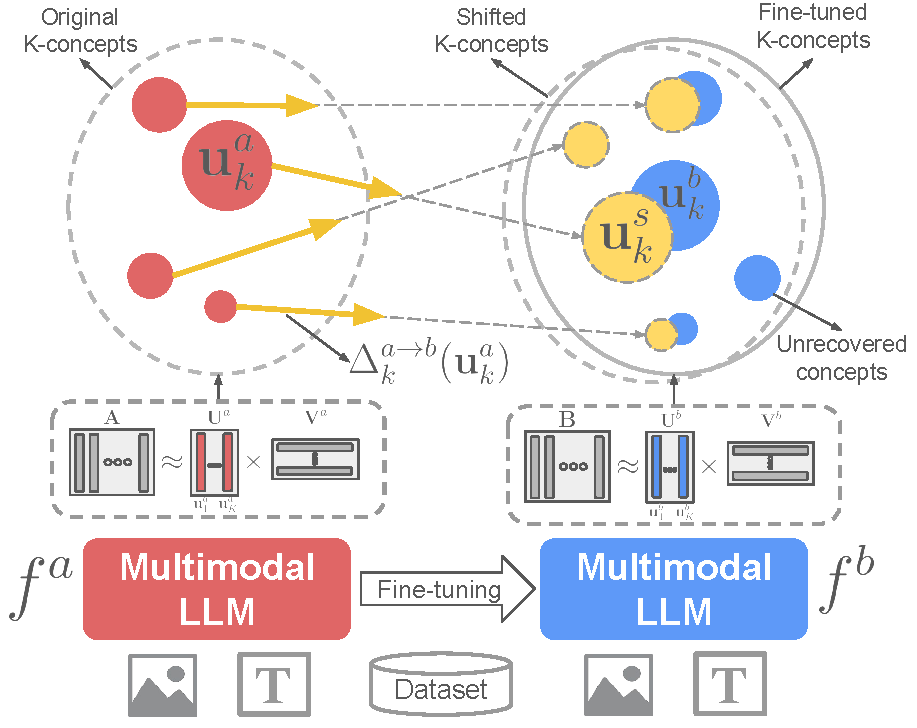
\includegraphics[width=\textwidth]{Figures/main/teaser.pdf}
    \end{minipage}%
\caption{\textbf{Analysis framework overview.} We analyse the  concepts representation change during fine-tuning and derive shift vectors that can recover most of the concept in the fine-tuned model.}
\label{fig:teaser}
\end{figure}


\paragraph{Concept-based explainability.} \label{sec:concept_based_method} To understand the internal representations of any given MLLM $f$, we leverage the approach introduced in \cite{parekh2024concept}.
Specifically, for a token of interest $\textit{TOI}$, we first extract the residual stream representations, after the $l-$th layer, $h_{(l)}^p = {f_l}(x)$ \cite{elhage2021mathematical} of a subset of samples $X_\textit{TOI} \subset \bmS$. $X_\textit{TOI}$ includes all the samples $x$ that contain $\textit{TOI}$ in both the ground truth and predicted response ($\textit{TOI} \in \hat{y} ; \hat{y} = f(x)$). For simplicity, given a sample $x_m$ the extracted hidden states (or features) corresponding to the $\textit{TOI}$ token is denoted as $\bm{z}_m = {f_l}(x_m) \in \reals^{D}$, where $D$ is the features dimension. Thus the features from all samples gives a feature matrix $\bm{Z} \in \reals^{D \times M}$ where $M=|X_\textit{TOI}|$. The feature matrix $\bm{Z}$ is then decomposed as $\bm{Z} \approx \bm{UV}$ to discover the encoded concepts. Here, $\bm{U} \in \mathbb{R}^{D \times K}$ is the matrix of $K$ concepts and $\bm{V} \in \mathbb{R}^{K \times M}$ represents the coefficients/activations of the samples projected onto these concepts. Each column $\bm{u}_k \in \bm{U}$ corresponds to a concept, while each column of $\bm{V}$ encodes the activation of these concepts for a given sample. %
Note that any given representation $f_l(x)$ can be projected on $\bm{U}$ to obtain its activation vector $\bm{v}(x) \in \reals^K$, i.e. $f_l(x) \approx \bm{U} \bm{v}(x)$.



Each extracted concept is interpreted through grounding in both image and text spaces. Specifically, the top $N_{\text{MAS}}$ most activating samples for the concept $\bm{u}_k$ represent its image grounding $\bm{X}_{\text{MAS}}$:
\begin{equation}
\label{eq:mas}
\bm{X}_{\text{MAS}}(\bm{u}_k) = \argmax_{\hat{X} \subset \bfX_t ,\; |\hat{X}| = N_{\text{MAS}}} \sum_{x \in \hat{X}} \left| \bm{v}_k (x) \right|,
\end{equation}
where $\bm{v}_k(x)$ refers to the the activation of $\bm{u}_k$ for image $x$. For text grounding, we decode the features using the unembedding matrix of the language model $W_U$ \cite{Belrose2023ElicitingLP,Langedijk2023DecoderLensLI,nostalgebraist2020interpreting,DBLP:journals/corr/abs-2310-16270}. Specifically, the operation $W_U \bm{u}_k \in \reals^{|\bmY|}$ produces logits over the vocabulary, and the top $N_{\text{grounding}}$ words with highest logits are extracted:

\begin{equation}
\label{eq:text_ground}
\bm{T}_{\text{words}}(\bm{u}_k) = \argmax_{\text{Top-}N_{\text{grounding}}} (W_U \bm{u}_k).
\end{equation}

We employ $K$-Means to learn our concept dictionaries. This is motivated by $K$-Means' simplicity, and straightforward arithmetic manipulation of the clusters/concepts it allows, making it a more suitable for our analysis.



\paragraph{Fine-tuning setup.} To develop a specialized model $f^b$ tailored for a particular task—or, specifically, for a set of target concepts—the original model $f^a$ is fine-tuned on samples that include a set of words, $\{w_1, \cdots, w_m\}$, associated with these target concepts. Our focus is on fine-tuning the LLM component, using Low-Rank Adaptation (LoRA) \cite{Hu2021LoRALA}, an approach known to deliver performance comparable to full model fine-tuning while being significantly more efficient \cite{liu2024improvedllava,laurenccon2024mattersidefics2}.
After finetuning, we extract feature matrices $\bm{A} \in \mathbb{R}^{D \times M^a}$ ($M^a=|X_\textit{TOI}^a|$) from $f^a$ and $\bm{B} \in \mathbb{R}^{D \times M^b}$ ($M^b=|X_\textit{TOI}^b|$) from $f^b$, which contain the set of residual stream representations composed of:
\begin{align*}
    \bm{a_i} = f_{l}^a(x^a_i), \quad \bm{b_j} = f_{l}^b(x^b_j),
\end{align*}
where $x^a_i \in X_\textit{TOI}^a$ and $x^b_j \in X_\textit{TOI}^b$ are samples where $\textit{TOI}$ is present in the ground truth and the response of both $f^a$ and $f^b$. Next, the matrices $\bm{A}$ and $\bm{B}$ are decomposed to extract the concepts each encodes as:
\begin{align*}
    A \approx \bm{U}^a \bm{V}^a , \quad B \approx \bm{U}^b \bm{V}^b ,
\end{align*}
where the hidden states of each sample can be represented as $\bm{a}_i = \bm{U}^a \bm{v}^a(x^a_i)$ and $\bm{b}_j = \bm{U}^b \bm{v}^b(x^b_j)$, \( \bm{U}^a \) with \( \bm{U}^b \) \( \in \mathbb{R}^{D \times K} \) representing the learned concepts $\{u^a_k\}_{k=1}^{K}, \{u^b_k\}_{k=1}^{K}$ respectively %
, and \( \bm{V}^a \) and \(\bm{V}^b\) \( \in \mathbb{R}^{K \times M} \) are the corresponding activations. 
Finally, we ground the concepts in the image modality (\Cref{eq:mas}) to obtain $\bm{X}_{k, \text{MAS}}^a$ and $\bm{X}_{k, \text{MAS}}^b$ as well as in the text modality (\Cref{eq:text_ground}) to obtain  $\bm{T}_{\text{words}}^a$ and $\bm{T}_{\text{words}}^b$.


\paragraph{Concepts similarity.}
To quantify the similarity of two concepts $u$ and $u^\prime$, we define \textit{Text Grounding Overlap} between them as:
\begin{equation}
   \text{T-Overlap}(\bm{u}, \bm{u}^\prime) = 100 \times \frac{ \left| \bm{T}_{\text{words}}(\bm{u}) \cap \bm{T}_{\text{words}}(\bm{u}^\prime) \right|}{ \left| \bm{T}_{\text{words}}(\bm{u})\right|}.
    \label{eq:text-overlap}
\end{equation}
One can similarly define the \textit{Image Grounding Overlap} and discussed in the Appendix.





\section{Fine-tuning and evolution of concept representations}
\label{sec:method}





We aim to study how fine-tuning process affects the concepts learned by the model. Then we try to recover the fine-tuned model concepts using shift vectors computed in the feature space.







\begin{figure}[t]
    \centering
    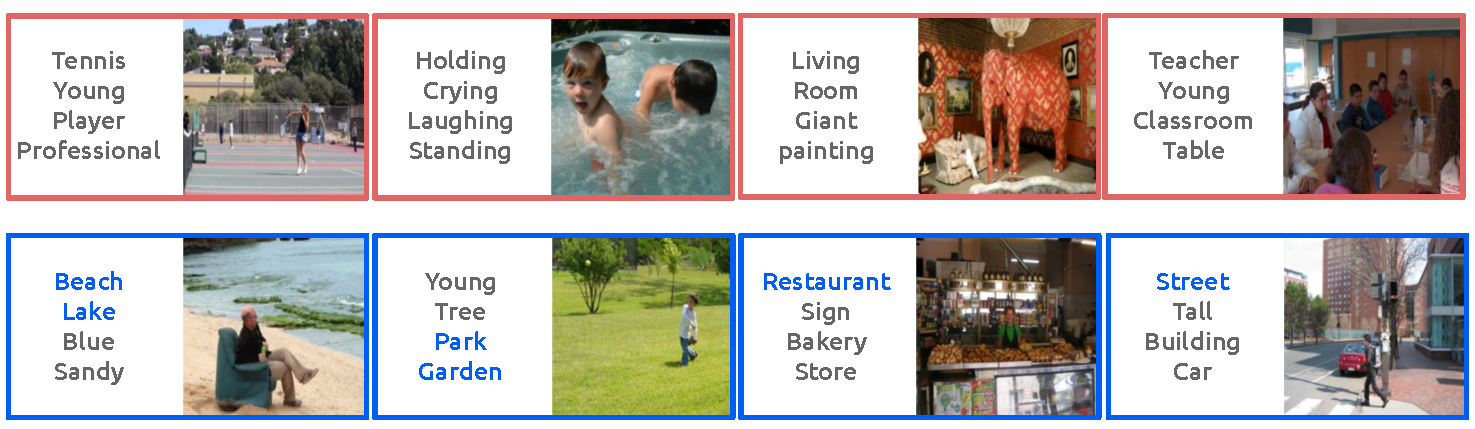
\includegraphics[width=1.0\linewidth]{Figures/Finetuing_Change_Concepts/several_concepts_VG_person_kmeans_40_boxes.pdf}
    \caption{\textbf{Concepts extracted from original and fine-tuned models}. Illustration of concepts groundings, for $\textit{TOI}= \text{person}$, extracted from $f^a$ (top),  and $f^b$ (bottom) which is fine-tuned to focus more on places. Notably, the concepts from $f^b$ exhibit a stronger association with places.}
    \label{fig:global_concept_change}
\end{figure}

\paragraph{Implementation details.} We focus on MLLMs with the architecture described in \Cref{sec:framework}. The image encoder \( f_V \) is a ViT-L/14 CLIP \cite{clip}, followed by a transformer-based connector that reduce the number of encoded visual tokens. The LLM \( f_{\text{LM}} \) is an OPT-6.7B model \cite{Zhang2022OPTOP} with 32 layers. We conduct our study in a controlled setups that consists of specializing the model on a target dataset. Specifically, we fine-tune on three different subsets of the Visual Genome dataset \cite{DBLP:journals/ijcv/KrishnaZGJHKCKL17}, related to places, colors, and sentiments (see App. A for more details).



\subsection{Impact of fine-tuning on learned concepts}
The fine-tuning process introduces changes in the overall structure of the learned concepts.
This change can be observed through the concepts groundings in both the text and image space (\Cref{fig:global_concept_change}). 

\begin{figure}[h]
    \centering
    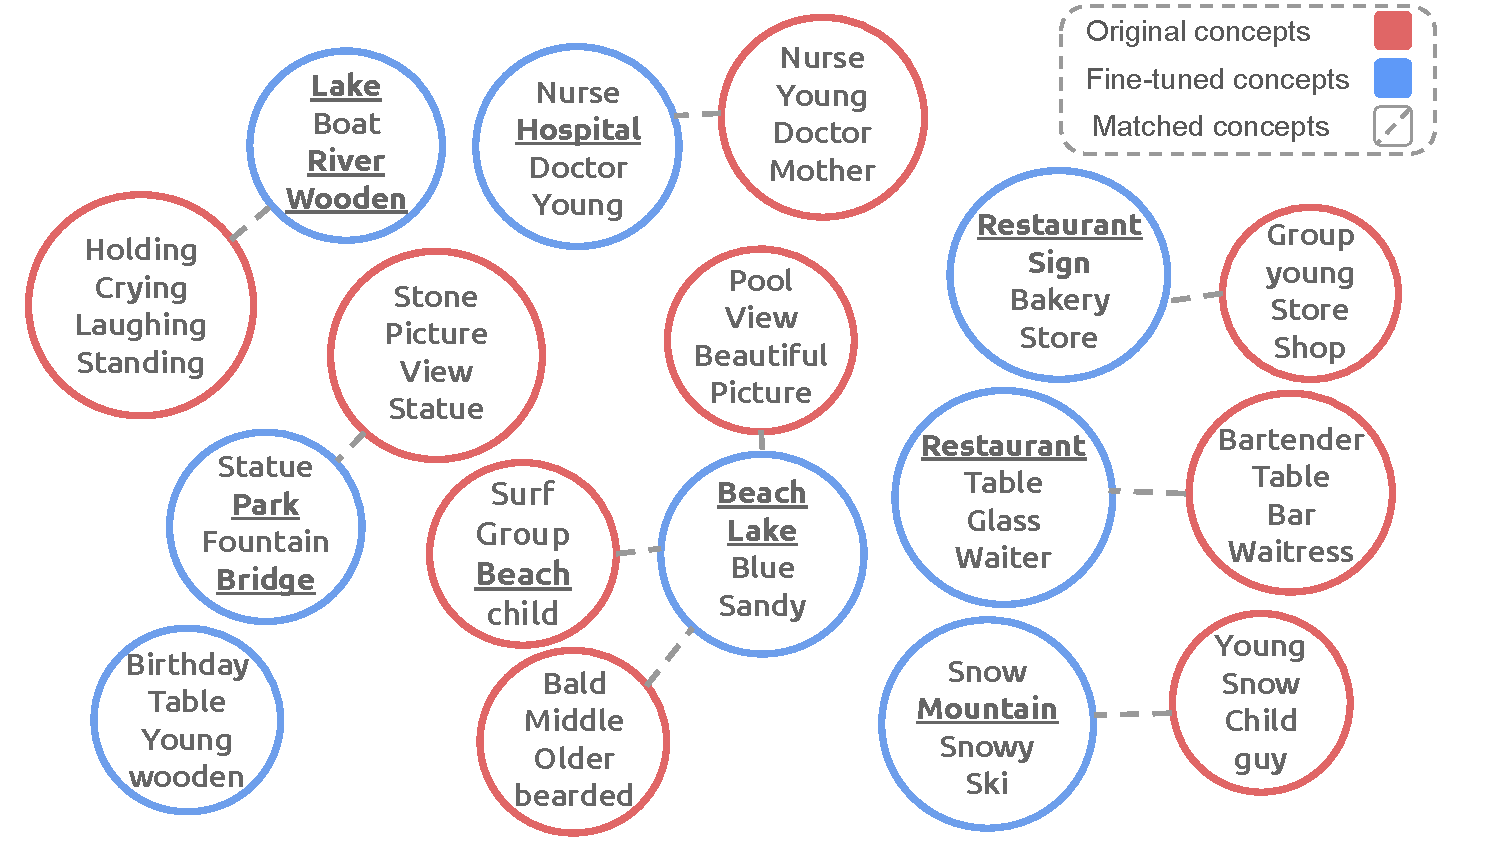
\includegraphics[width=0.95\linewidth]{Figures/Finetuing_Change_Concepts/bubble_words.pdf}
    \caption{\textbf{Concepts text grounding change after fine-tuning.} Illustration of text grounding for concepts ($\textit{TOI}= \text{person}$) from $f^a$ and their match from $f^b$, after fine-tuning to focus more on places.
    }
    \label{fig:bubble_words}
\end{figure}
\vspace{-0.8cm}

\paragraph{Matched concepts.} To analyze how each concept changes after fine-tuning, we focus on each concept and its match (see \Cref{fig:bubble_words}). Specifically, we define a matching function \( m: i \rightarrow j^* \) which associates each concept vector \( \bm{u}^a_{i} \) in set \( \bm{U}^a \) to its closest vector \( \bm{u}^b_{j^*} \) in set \( \bm{U}^b \) based on cosine similarity, i.e:
\begin{align}
& m(i) = \argmax_{\bm{u}^b_{j} \in \bm{U}_b} \text{cos}(\bm{u}^a_{i}, \bm{u}^b_{j}), \;  \text{cos}(\bm{u}^a_{i}, \bm{u}^b_{j}) = \frac{\bm{u}^a_{i} \cdot \bm{u}^b_{j}}{\|\bm{u}^a_{i}\| \|\bm{u}^b_{j}\|}
\end{align}




    






\begin{figure}[h]
    \centering
    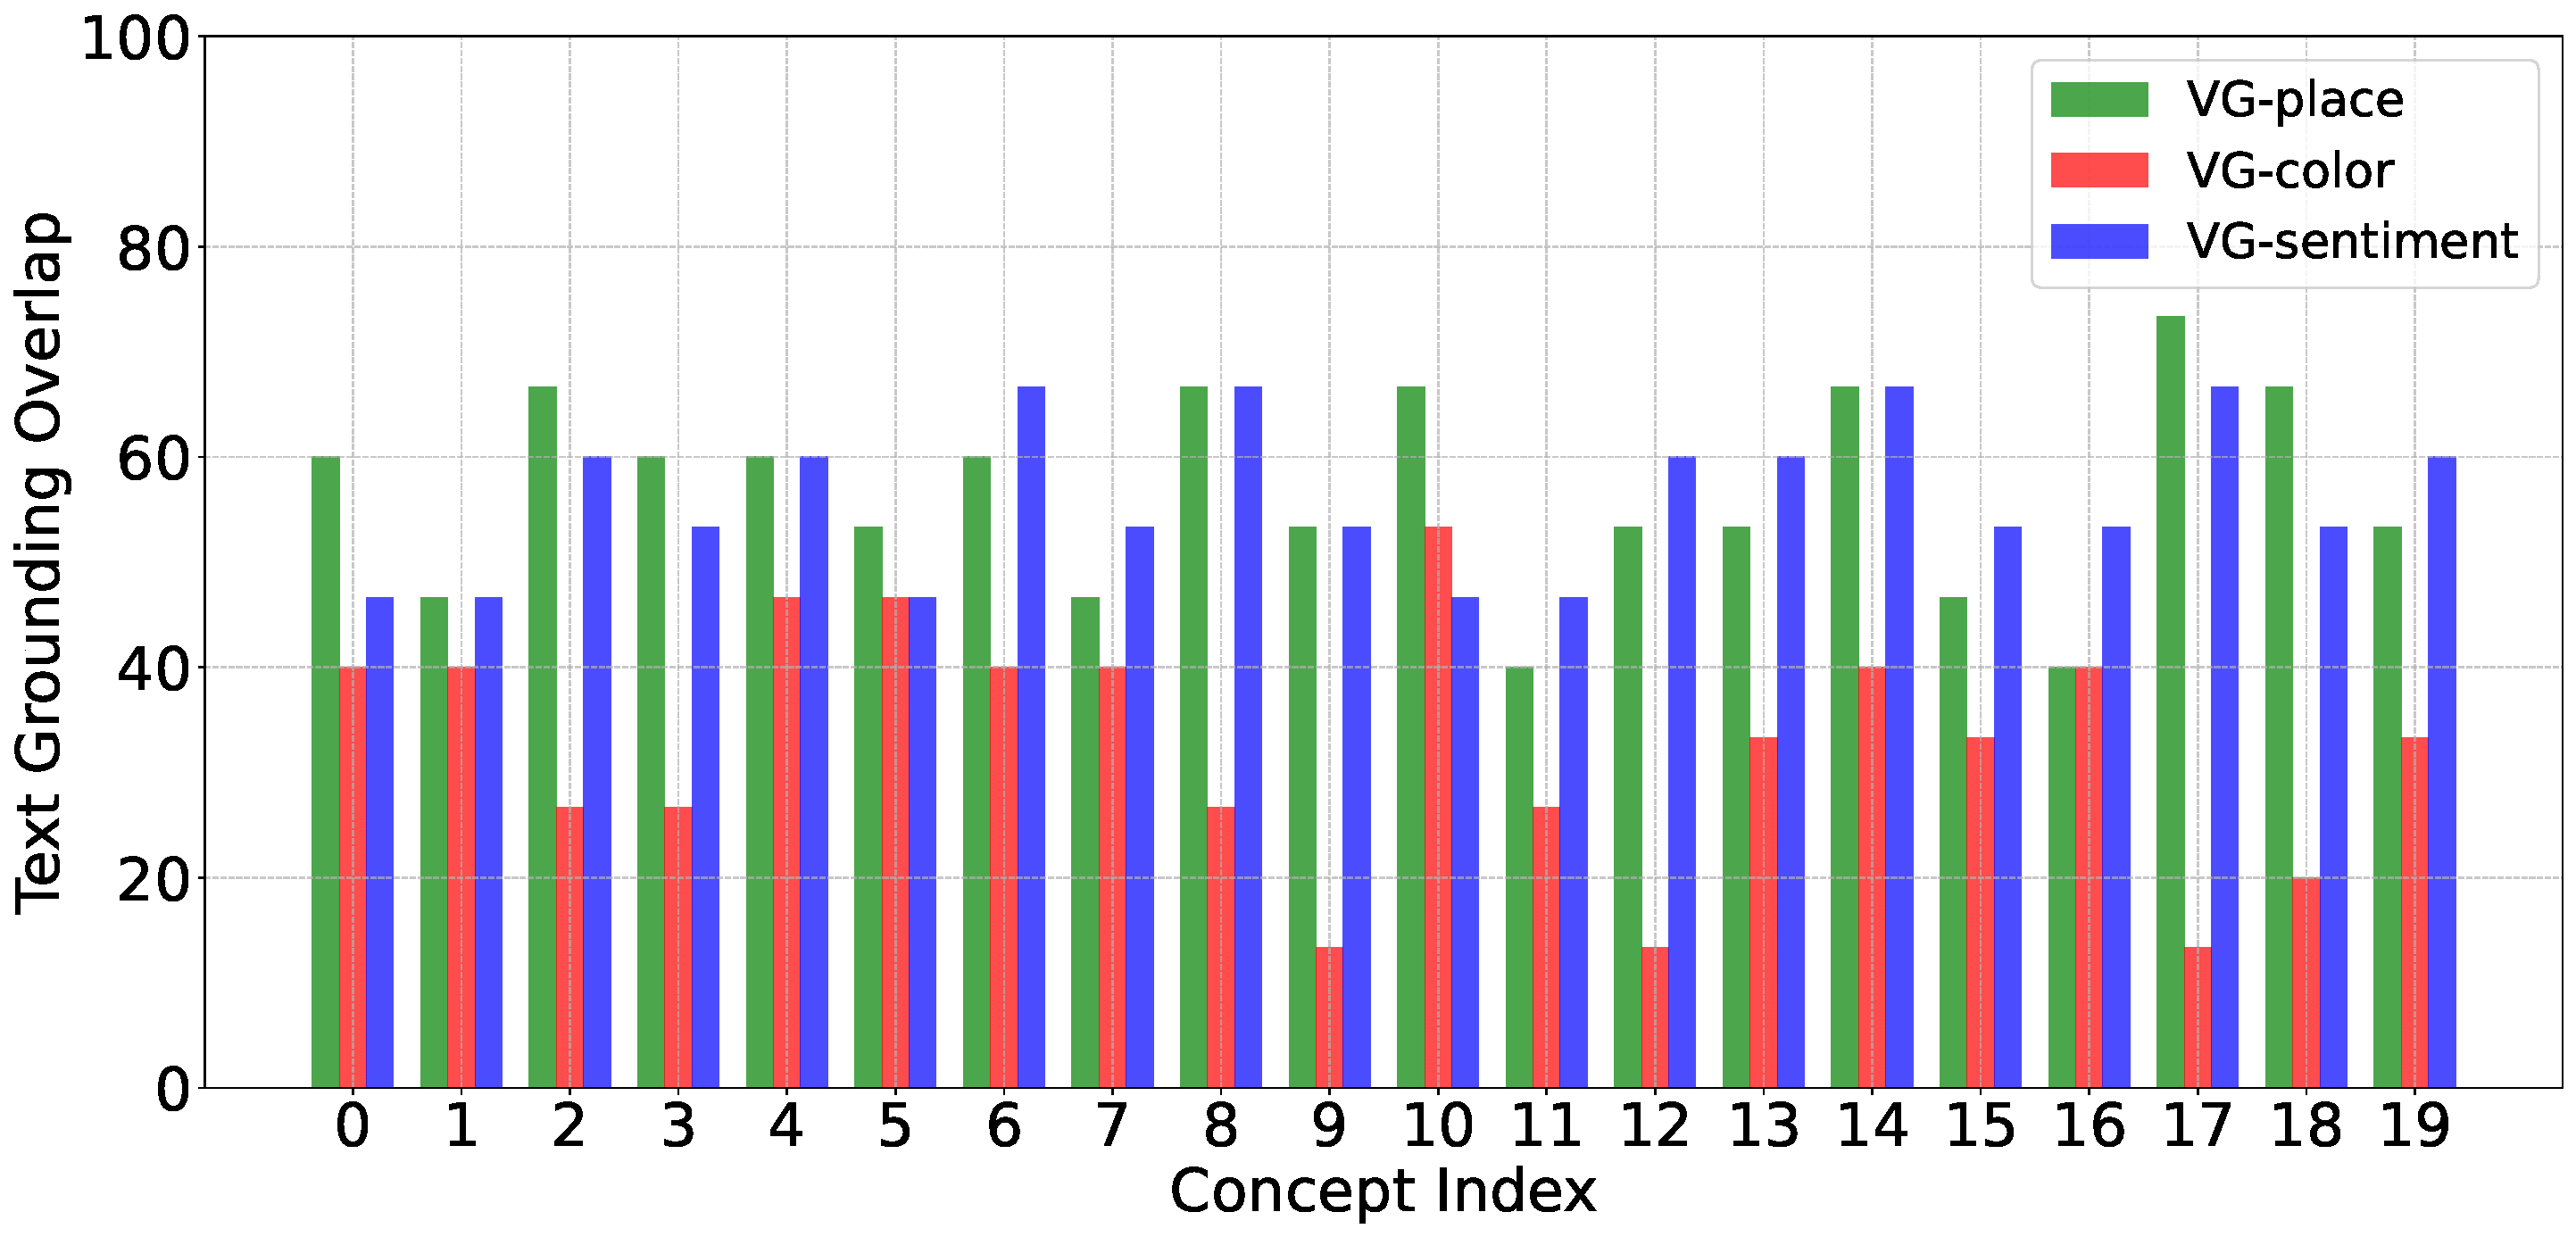
\includegraphics[width=1\linewidth]{Figures/Finetuing_Change_Concepts/VG_dog_bars_best_matched_to_original_appearance.pdf}
    \caption{\textbf{Text grounding overlap between original and fine-tuned models.} Illustration of $\text{T-Overlap}$ between original and matched fine-tuned model concepts.
    }
    \label{fig:evolution_intersection_w_original_grounding}
\end{figure}



\paragraph{Concept evolution.} 
To quantify how much a concept \( \bm{u}^a_{i} \in \bm{U}^a \) is changed after fine-tuning, we compute the overlap between its grounding words and those of its closest matching concept from the fine-tuned model \( \bm{U}^b \). Specifically, we compute $\text{T-Overlap}(\bm{u}^a_i , \bm{u}^b_{m(i)})$ (\Cref{eq:text-overlap}) for all the concepts $i \in \{1, \dots , K\}$, and visualize them for different fine-tunings in \Cref{fig:evolution_intersection_w_original_grounding}.
We observe varying rates of change across different concepts and fine-tunings. This might be due to the difference in the fine-tuning dataset size, complexity, or similarity to the original dataset.
It also highlights 2 main behaviors, detailed as follows:
\begin{itemize}
    \item \textit{Concepts that are refined.} This group contains the concepts that slightly change to be more specialized towards the fine-tuning task (\Cref{fig:shift}). These concepts exhibit a relatively high ($\text{T-Overlap}(\bm{u}^a_i , \bm{u}^b_{m(i)})$). 

     \item \textit{Concepts that change completely.}   This group contains the concepts that emerge (\Cref{fig:appearance}) or disappear (\Cref{fig:disappearance}) in the fine-tuned model. New concepts emerge in the fine-tuned model, likely due to the introduction of novel patterns or relationships not present in the original model. These concepts exhibit a relatively low ($\text{T-Overlap}(\bm{u}^a_i , \bm{u}^b_{m(i)})$).
     
\end{itemize}













    

        
        
        



        
\begin{figure}[!h]

    \centering
    
    \subfloat[\scriptsize{\textbf{Refined concepts:} fine-tuned model concepts show more grounding to places.}]{
        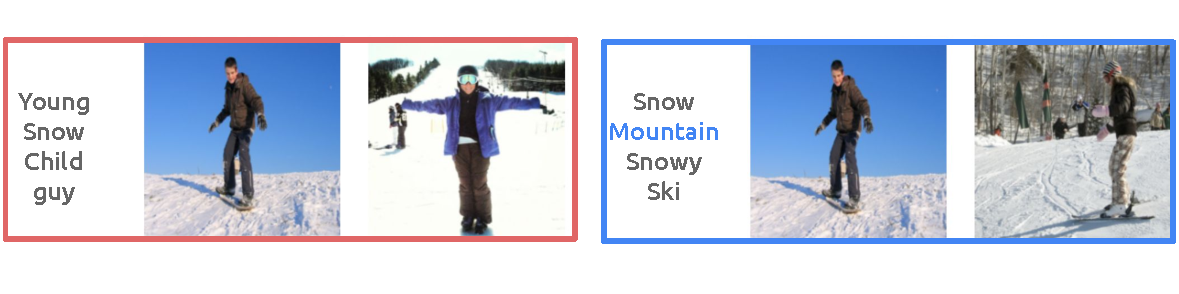
\includegraphics[width=0.45\textwidth]{Figures/Finetuing_Change_Concepts/fig6_refined.pdf}
        \label{fig:shift}
    }


    \subfloat[\scriptsize{\textbf{Emerged concepts:} only fine-tuned model concepts show groundings related to places.}
    ]{
        
\includegraphics[width=0.45\textwidth]{Figures/Finetuing_Change_Concepts/fig6_appear.pdf}
        \label{fig:appearance}
    }


    \subfloat[\scriptsize{\textbf{Diminished concepts:} original model concepts (actions) disappeared after fine-tuning.}
    ]{
        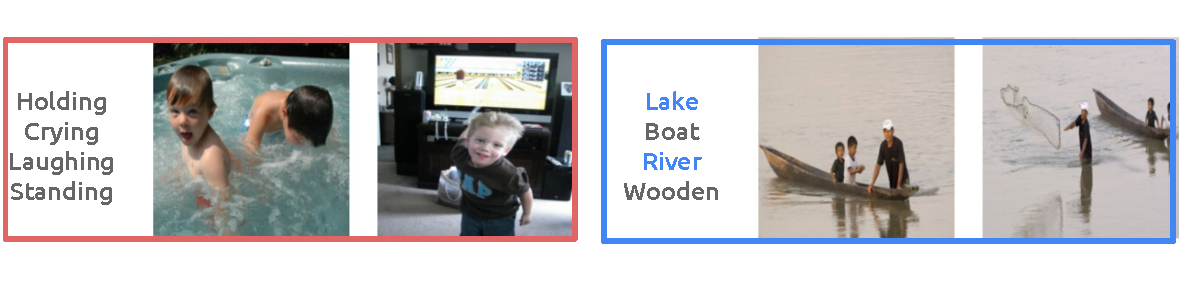
\includegraphics[width=0.45\textwidth]{Figures/Finetuing_Change_Concepts/fig6_disappear.pdf}
        \label{fig:disappearance}
    }
    \caption{\textbf{Concepts evolve differently due to fine-tuning.} Left: concepts extracted from the original model $f^a$. Right: concept extracted from $f^b$, fine-tuned to focus on places. Each concept is grounded in image and text. 
    }
    \label{fig:qualitative_change_concepts}
\end{figure}




We also notice that the $\text{T-Overlap}$ decreases with the number of training iterations, indicating that fine-tuning leads to deviation from original model concepts (see App. A for more details).


\subsection{Recovering concepts in fine-tuned model via shift vectors}

In this section, we study if the learned concepts in the fine-tuned model can be recovered from the original model concepts, without any training or decomposition. In particular, we propose to characterize the change in original concepts due to fine-tuning as linear directions in the feature space, referred to these as \emph{concept shift vectors.} 


\paragraph{Shifting original model concepts.} To compute the concept shift vectors, we first associate each concept $\bm{u}^a_k$ in the original model with a subset of samples common to the analysis of both $f^a$ and $f^b$. Specifically, projecting the representation of each sample $x_m \in \bm{X}_{TOI}^{a} \cap \bm{X}_{TOI}^{b}$ on $\bm{U}^a$ and selecting those that activate $\bm{u}^a_k$ the most:
$$\bm{A}_{k} = \{ m \;|\; k = \argmax_{i} \, \left|\bm{v}^a_i(x_m) \right| \}.$$ 
For each sample $x_m, m \in \bm{A}_k$ we define $\delta^{a \to b}_m = \bm{b}_m - \bm{a}_m$ as the change in its representation from $f^a$ to $f^b$. To compute the concept shift vector $\bm{\Delta}_k^{a \to b}(\bm{u}^a_k)$ associated with $\bm{u}^a_k$, we aggregate shifts of its associated samples specified by $\bm{A}_k$:
\begin{align}
    \bm{\Delta}_k^{a \to b}(\bm{u}^a_k) &= \frac{1}{|\bm{A}_{k}|} \sum_{m \in \bm{A}_{k}} \delta^{a \to b}_m = \frac{1}{|\bm{A}_{k}|} \sum_{m \in \bm{A}_{k}} (\bm{b}_m - \bm{a}_m) \nonumber
\end{align}
The concept shift vector is used to shift each concept in the original model $\bm{u}^a_k$ to obtain the shifted concept $\bm{u}^s_k$:
\begin{equation}
    \bm{u}^s_k = \bm{u}^a_k + \alpha \; \bm{\Delta}_k^{a \to b}(\bm{u}^a_k),
\end{equation}
where $\alpha$ is a coefficient to control the shift magnitude. Unless otherwise stated, we use $\alpha=1$ as the default magnitude of shift. It is worth noting that given the concept shift vectors, the computation of shifted concepts does not rely on accessing the fine-tuned model. 

    
    


\paragraph{Evaluating fine-tuned concept recovery.} To study if the fine-tuned concepts $\bm{U}^b$ can be recovered from the original ones $\bm{U}^a$, we first establish a matching ($m: i \rightarrow j$) between the set of original $\{\bm{u}^a_i\}_{i=1}^K$ and fine-tuned concepts $\{\bm{u}^b_j\}_{j=1}^K$. For systematic evaluation of recovery of all fine-tuned concepts, we constrain $m$ to be bijective (see App. A for more details). Finally, we evaluate how well a shifted concept $\bm{u}^s_k$ is similar to its match $\bm{u}^b_{m(k)}$ using the overlap metrics. \Cref{fig:recovery-individual} shows the results of recovering the fine-tuned concepts for models fine-tuned on different subsets of the VG dataset (place, color, sentiment). We compare the text grounding overlap between the shifted $u^s_k$ and fine-tuned concepts $u^b_{m(k)}$. We use the overlap between the original concepts $u^a_k$ with the fine-tuned ones as a baseline. As we can see, most shifted concepts exhibit higher overlap than the original ones. Many of them have very high overlap close to 100\% (full recovery).












    
    

\begin{figure}
    \centering
    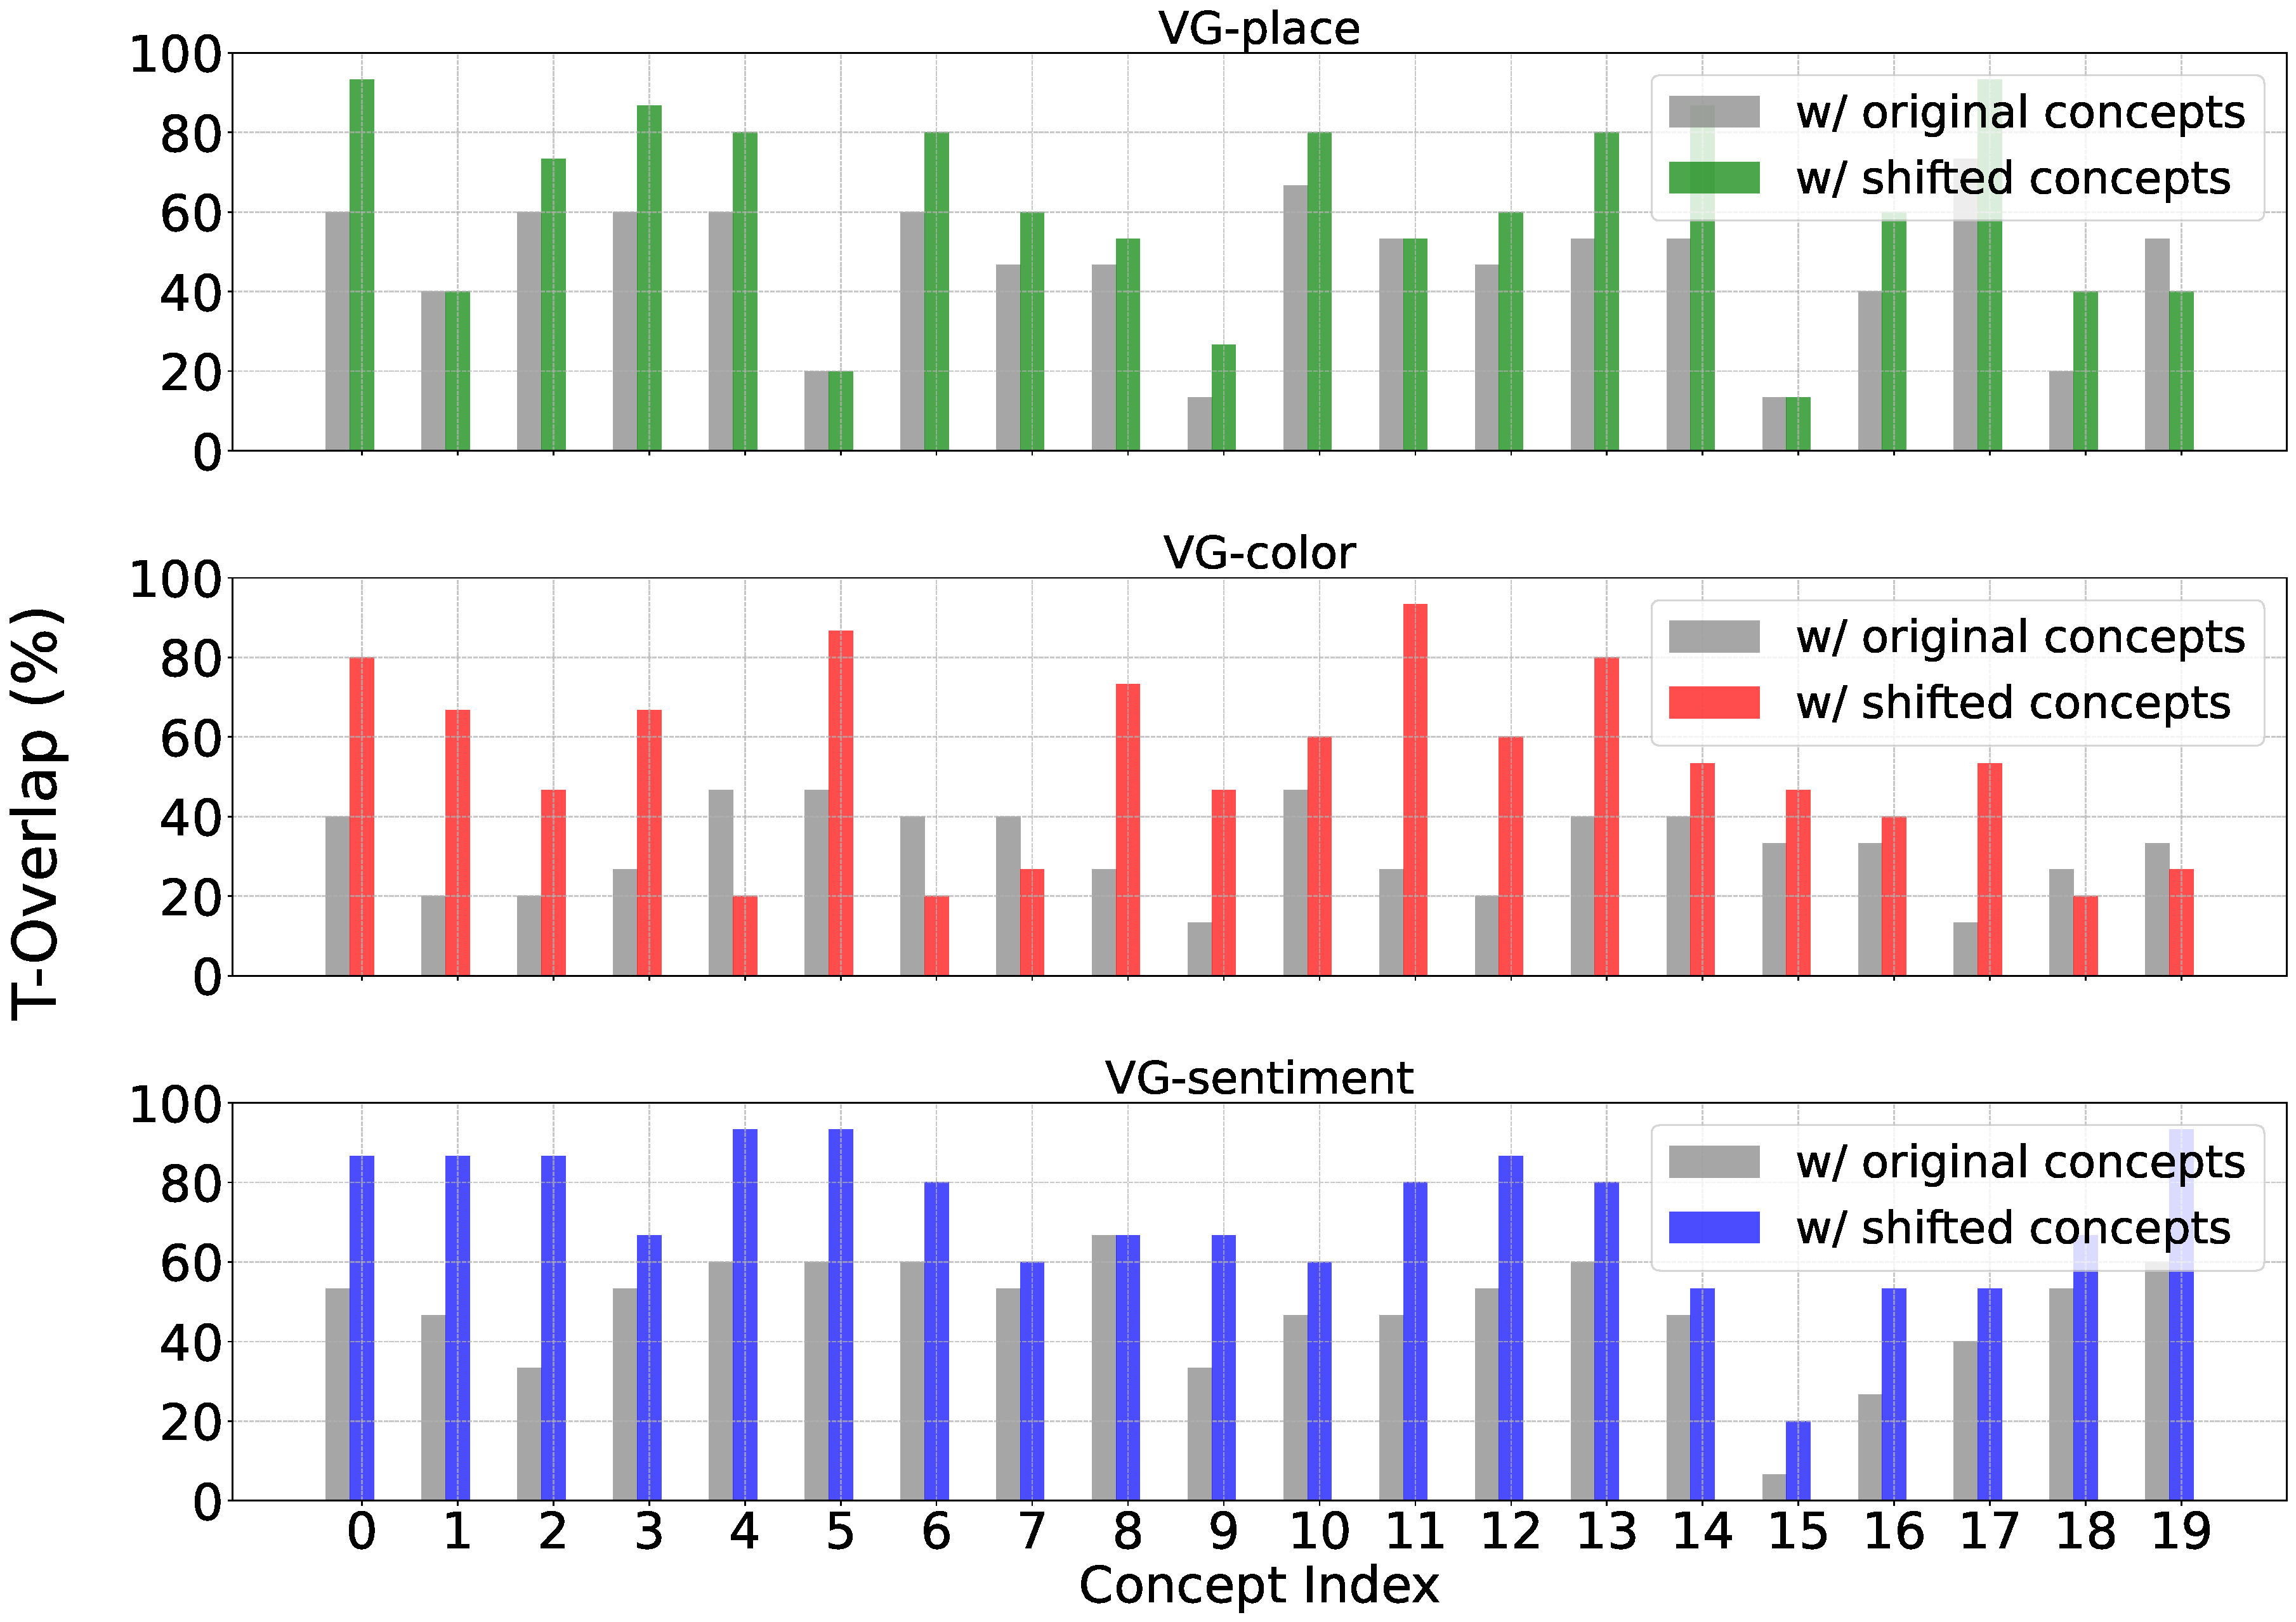
\includegraphics[width=1\linewidth]{Figures/Shifting_concepts_recovery/VG_bars_coco_dog_grounding_recovery_words.pdf}

    \caption{\textbf{Recovering fine-tuned model concepts}. For each matched fine-tuned concept we report its text grounding overlap with the original concept and the shifted concept. Model fine-tuned on: places (top), colors (middle) and sentiments (bottom).}
    \label{fig:recovery-individual}
\end{figure}




\begin{figure}[h]
    \centering
    \begin{minipage}{\linewidth}
    \centering
        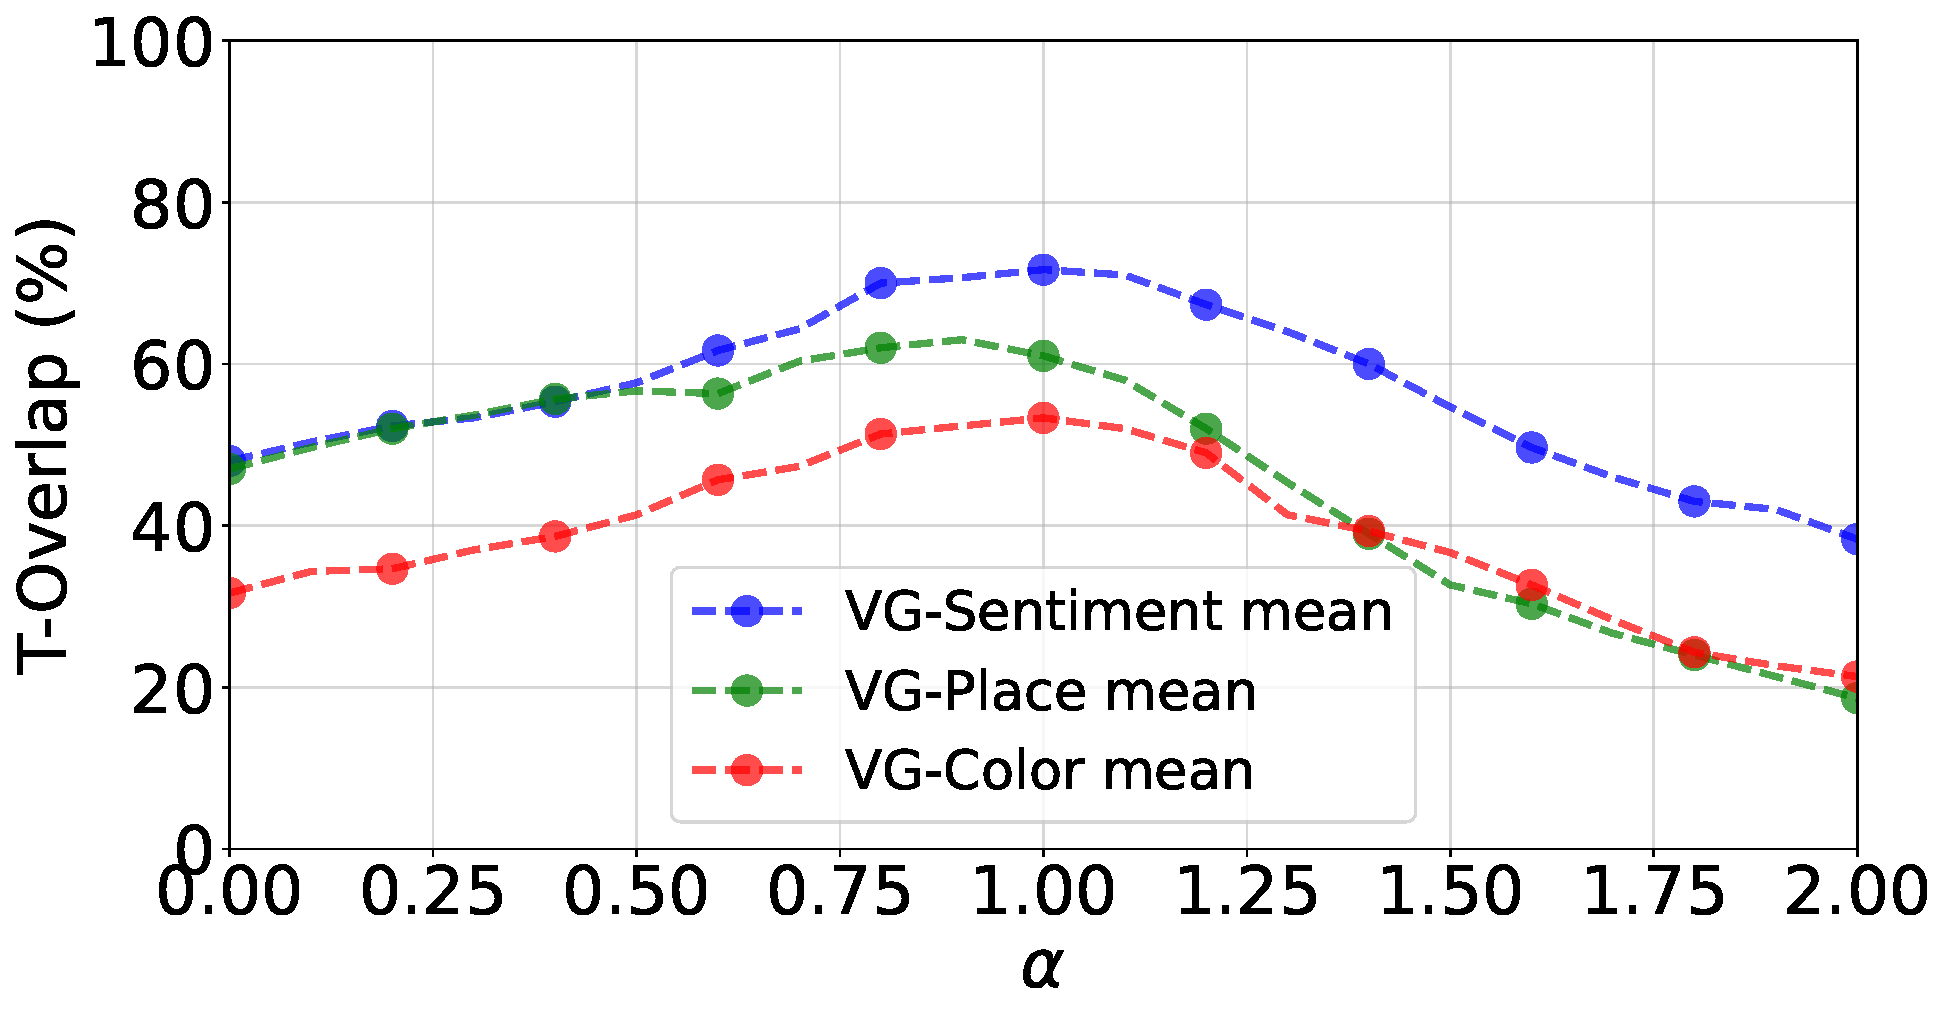
\includegraphics[width=0.85\linewidth]{Figures/mean_recovery_all.pdf}
    \end{minipage}
\caption{\textbf{Shift magnitude ($\alpha$) and recovering fine-tuned model concepts.} Illustration of the average of $\text{T-Overlap}$ between shifted and matched fine-tuned concepts when varying the shift magnitude.}
\label{fig:mean_recovery}
\end{figure}
\paragraph{Shift magnitude ($\alpha$) and concepts recovery.}
We also study the amount of recovery for shifted concepts, obtained with different shift magnitudes $\alpha$. We report the average recovery over $K=20$ concepts for each fine-tuning task for different $\alpha$ values in \Cref{fig:mean_recovery}. Note that $\alpha=0$ corresponds to original concepts. $\alpha=1$ generally corresponds to the most optimal value of shift magnitude (color, sentiment fine-tuning) or very close to the optimal value (place fine-tuning). This indicates that simply adding the mean shift vector to the original concept without scaling, generally offers the best possibility to recover the fine-tuned concepts. 

\begin{figure}[h]
    \centering
    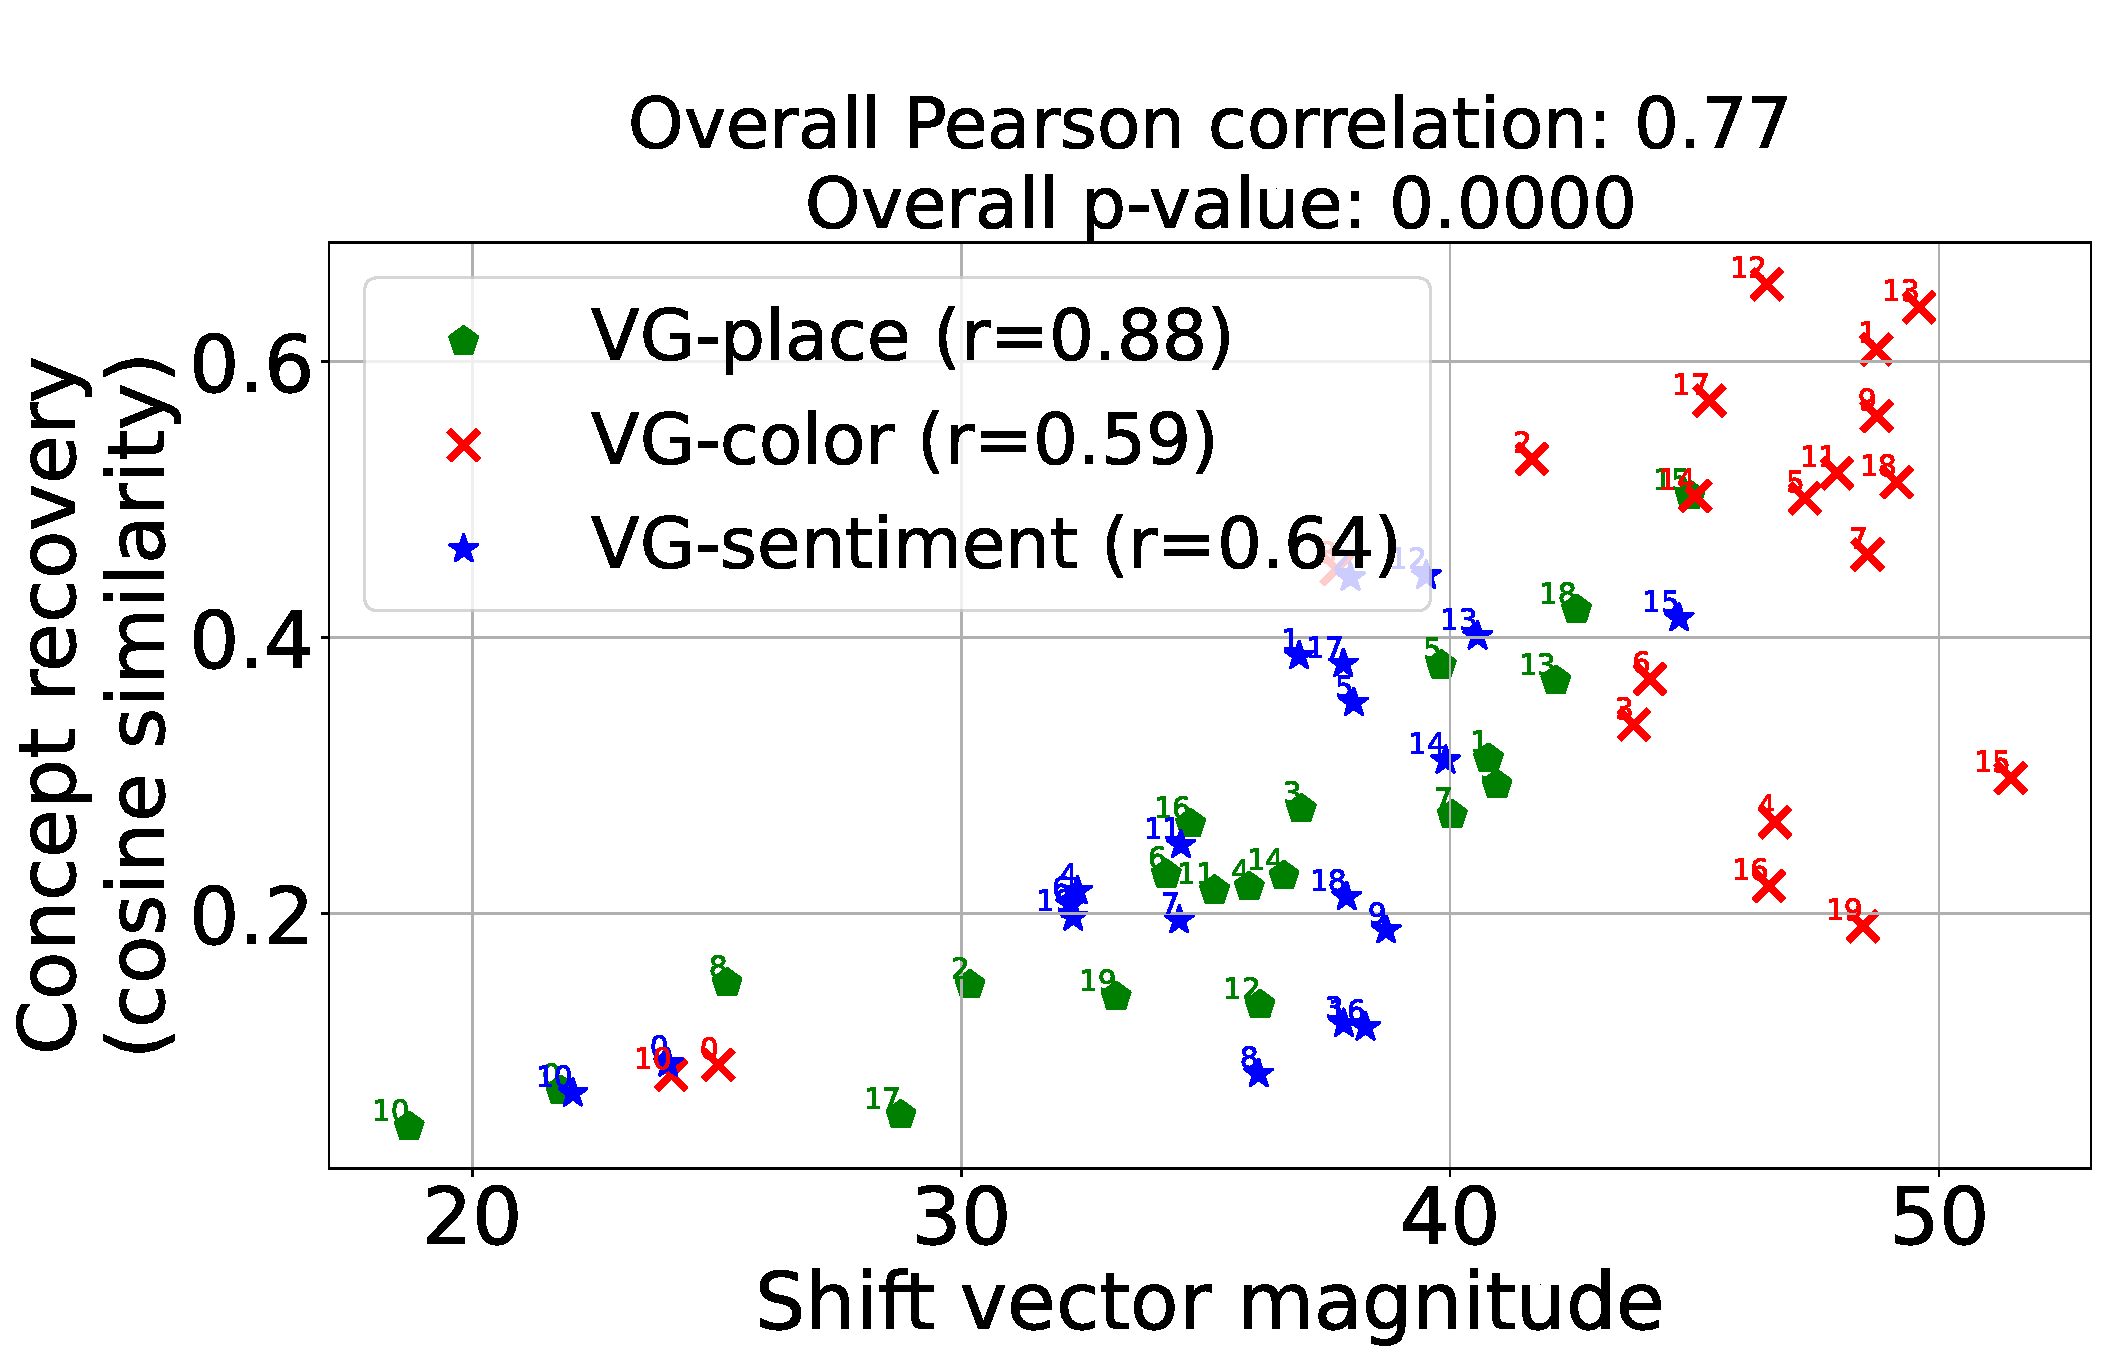
\includegraphics[width=0.9\linewidth]{Figures/Shifting_concepts_recovery/dog_mag_mean_shift_cosine_improve_v2.pdf}
    \caption{\textbf{Correlation between shift vector magnitudes and concept recovery.} Each point corresponds to an original concept from models fine-tuned on 3 VG subsets. The higher the shift vector magnitude the better the concept recovery.}
    \label{fig:correlation_shift_mag_recovery}
\end{figure}
\paragraph{Which concepts are recovered?} We examine the potential correlation between the computed concept shift vectors and the recovery of concepts in the fine-tuned model. We hypothesize that if samples related to an original concept consistently and significantly shift toward the corresponding fine-tuned model concepts, the shift vector, computed based on these samples, should be more effective at recovering this concept. Assuming that individual shifts $\delta_m^{a \rightarrow b}$ associated with each original concept tend to have similar magnitudes, their aggregation $\Delta_k^{a \to b}$ should have a higher magnitude when they are aligned.  We validate that this assumption is reasonable for most concepts in our analysis (App. A). 

For discovered concepts across all three fine-tuning tasks, we measure the correlation between the magnitude of the concept shift vectors $||\Delta_k^{a \to b}||$ and concepts recovery, here, measured as the cosine similarity between the shifted and matched fine-tuned concept. For a given shifted concept $\bm{u}^s_k$, this recovery (CR) is calculated as:
\begin{align}
\text{CR}_k = \frac{\text{cos}(\bm{u}^b_{m(k)}, \bm{u}^s_{k})-\text{cos}(\bm{u}^b_{m(k)}, \bm{u}^a_{k})}{\text{cos}(\bm{u}^b_{m(k)}, \bm{u}^a_{k})}
\end{align}
This is illustrated in \Cref{fig:correlation_shift_mag_recovery}, where we observe a noticeable correlation between the two quantities, which further strengthens our hypothesis.  





















\begin{figure}[!h]
    \centering
    \begin{minipage}{0.9\linewidth}
    \centering        
        \begin{minipage}{\linewidth}
            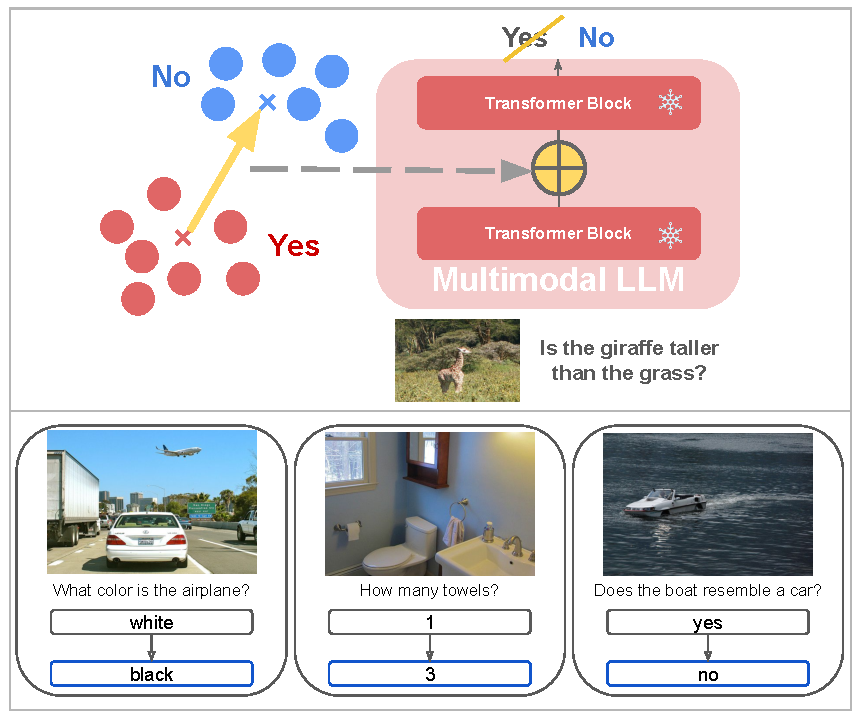
\includegraphics[width=1.0\textwidth]{Figures/main/teaser_steering.pdf}
        \end{minipage}%
    \end{minipage}
\caption{\textbf{Steering MLLMs answers.} \textbf{Top}: overview of the steering framework. We add a steering vector to the residual stream of MLLMs to change its response. \textbf{Bottom}: Each example corresponds to different steering vector that change a specific original answer (\emph{e.g.}, white) to a \textcolor{NavyBlue}{target} one (\emph{e.g.}, black).}
\label{fig:model_steering_qual_change_answers_main}
\end{figure}



\section{Fine-grained multimodal LLM steering} 
\label{sec:model_steering}
Model steering (see \Cref{fig:model_steering_qual_change_answers_main}) refers to guiding the model outputs towards desired outcomes by modifying the features without altering the model weights. Here, we investigate this technique, focusing on large multimodal models for visual question-answering and image captioning tasks. We provide additional qualitative results and ablation study in App. B.


\paragraph{Motivation.} In the previous sections, we demonstrate the feasibility of recovering target concepts in fine-tuned models by shifting the original model features along shift vectors. In addition, we find that the features related to different concepts are almost linearly separable (\Cref{fig:model_steering_qual_pca_concepts_samples}), and this becomes more prominent in deeper layers. This validates the linear representation hypothesis for MLLMs, previously studied for LLMs \cite{park2024the,nanda_othello_2023}. Finally, model steering might be an alternative method to avoid costly fine-tuning.

\begin{figure}[h]
    \centering
    \begin{minipage}{1\linewidth}
    \centering
        \begin{minipage}{0.2\linewidth}
            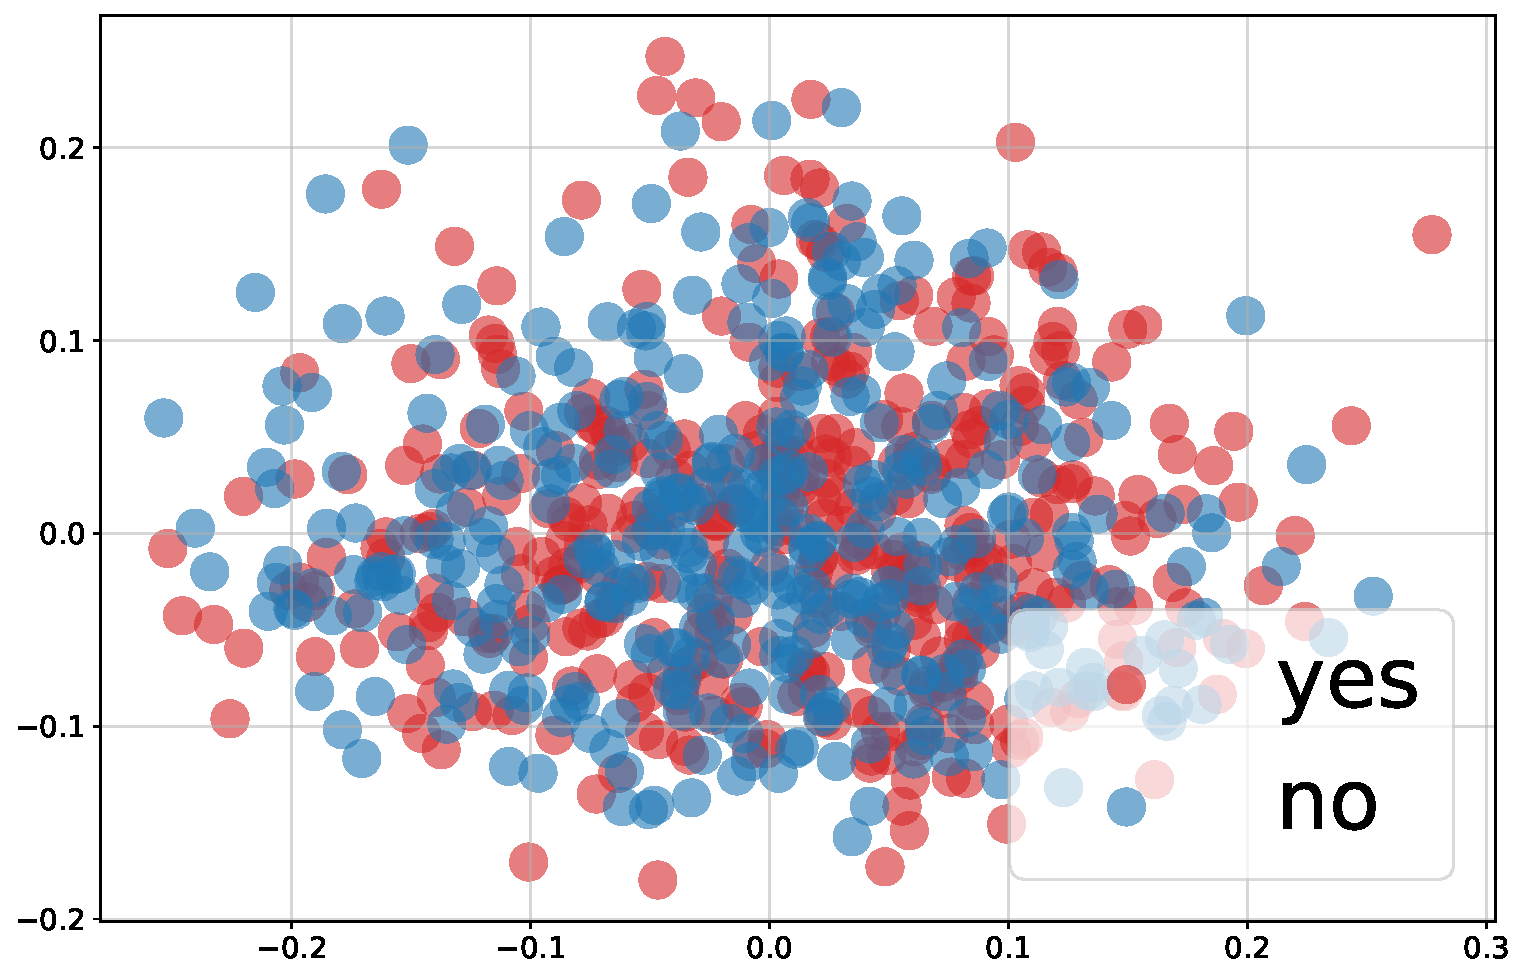
\includegraphics[width=1.0\textwidth]{Figures/model_steering/pca/pca_shift_of_means_llava_1_yes_to_no.pdf}
            \caption*{\small{$l=1$}}
        \end{minipage}%
        \begin{minipage}{0.2\linewidth}
            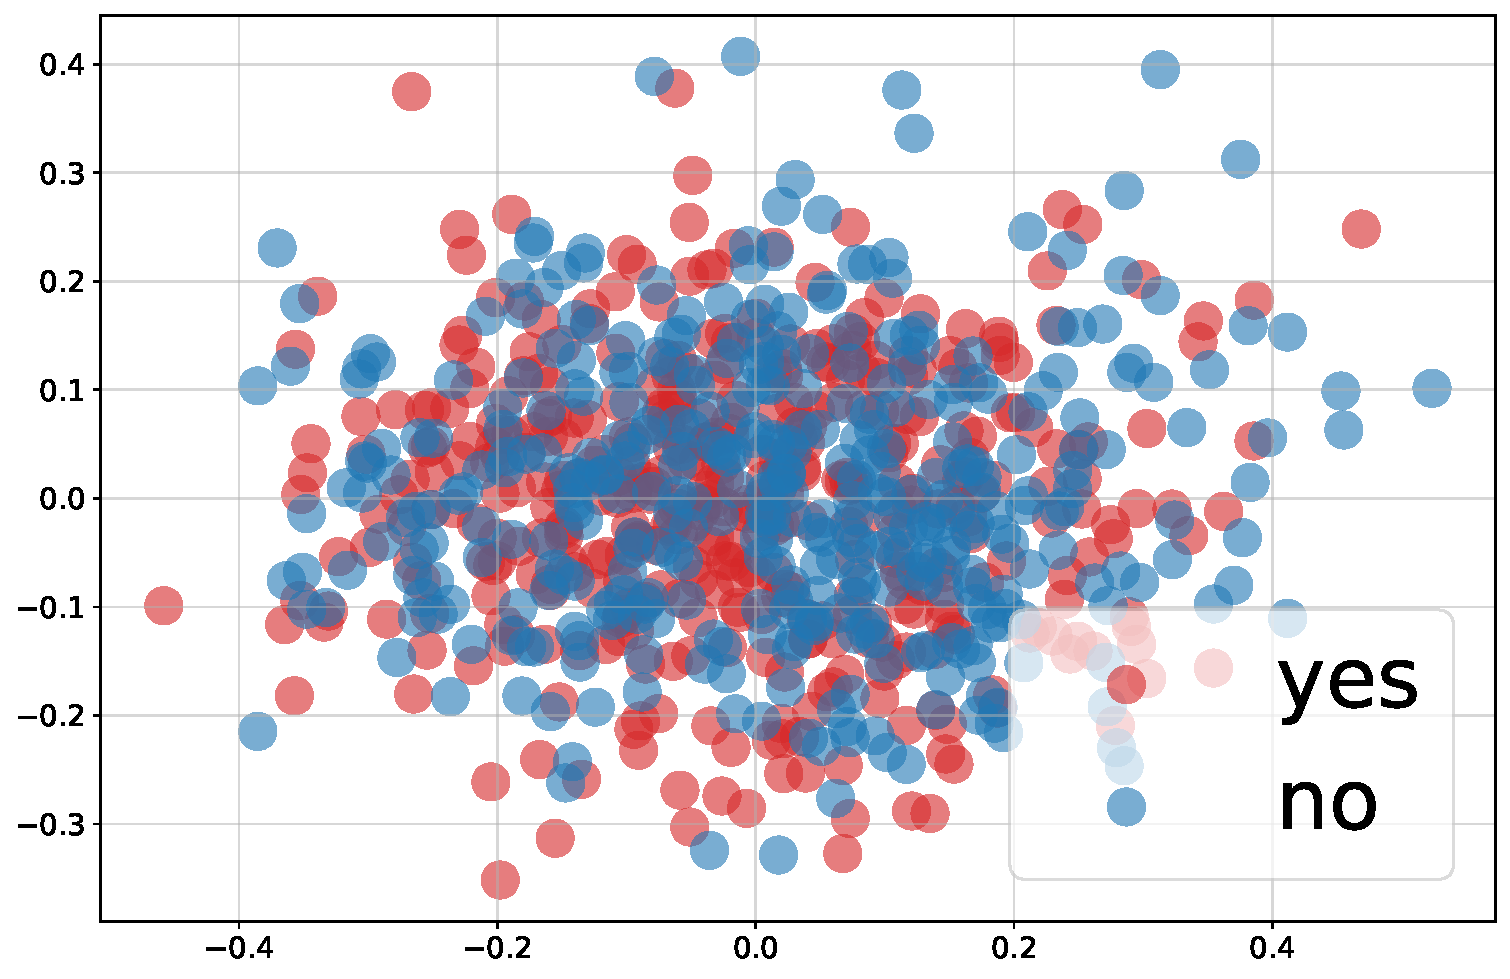
\includegraphics[width=1.0\textwidth]{Figures/model_steering/pca/pca_shift_of_means_llava_3_yes_to_no.pdf}
            \caption*{\small{$l=3$}}
        \end{minipage}%
        \begin{minipage}{0.2\linewidth}
            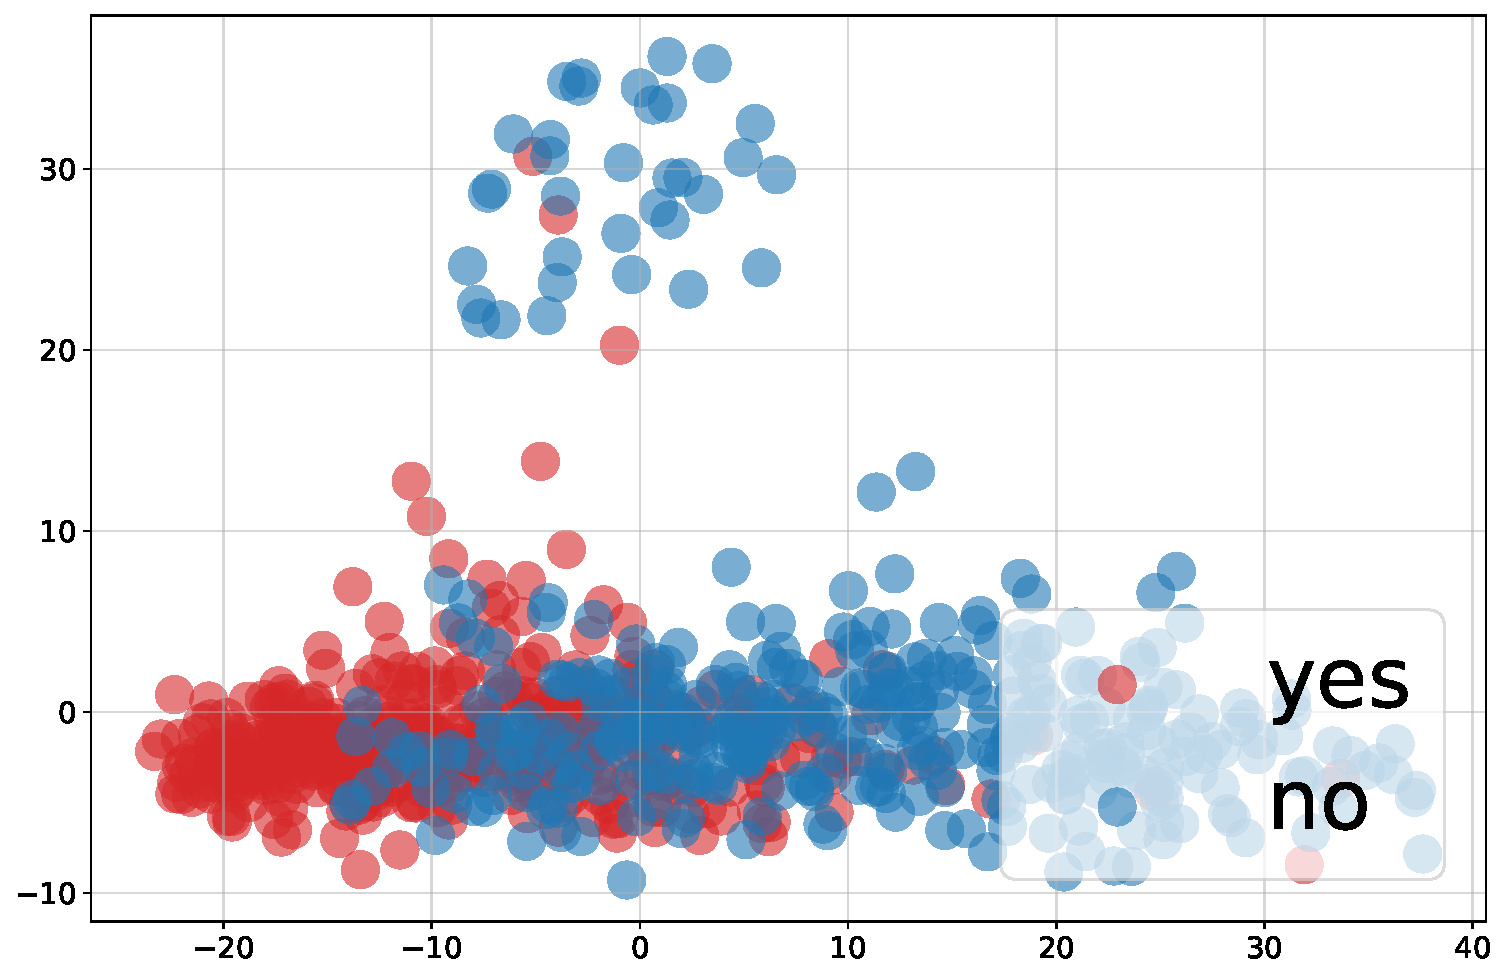
\includegraphics[width=1.0\textwidth]{Figures/model_steering/pca/pca_shift_of_means_llava_19_yes_to_no.pdf}
            \caption*{\small{$l=19$}}
        \end{minipage}%
        \begin{minipage}{0.2\linewidth}
            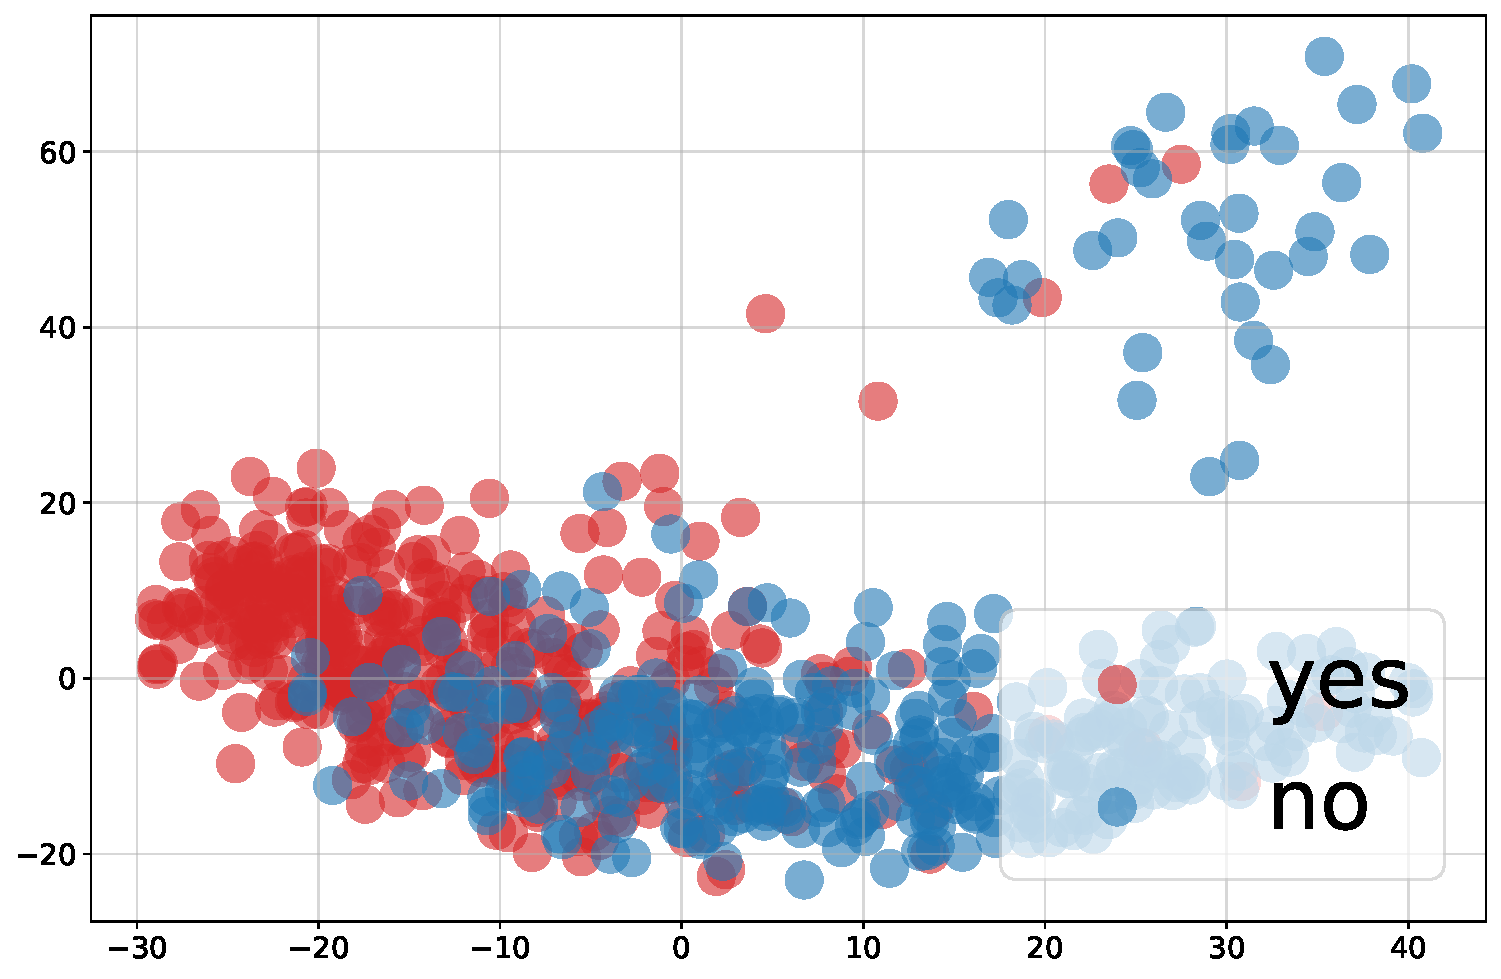
\includegraphics[width=1.0\textwidth]{Figures/model_steering/pca/pca_shift_of_means_llava_25_yes_to_no.pdf}
            \caption*{\small{$l=25$}}
        \end{minipage}%
        \begin{minipage}{0.2\linewidth}
            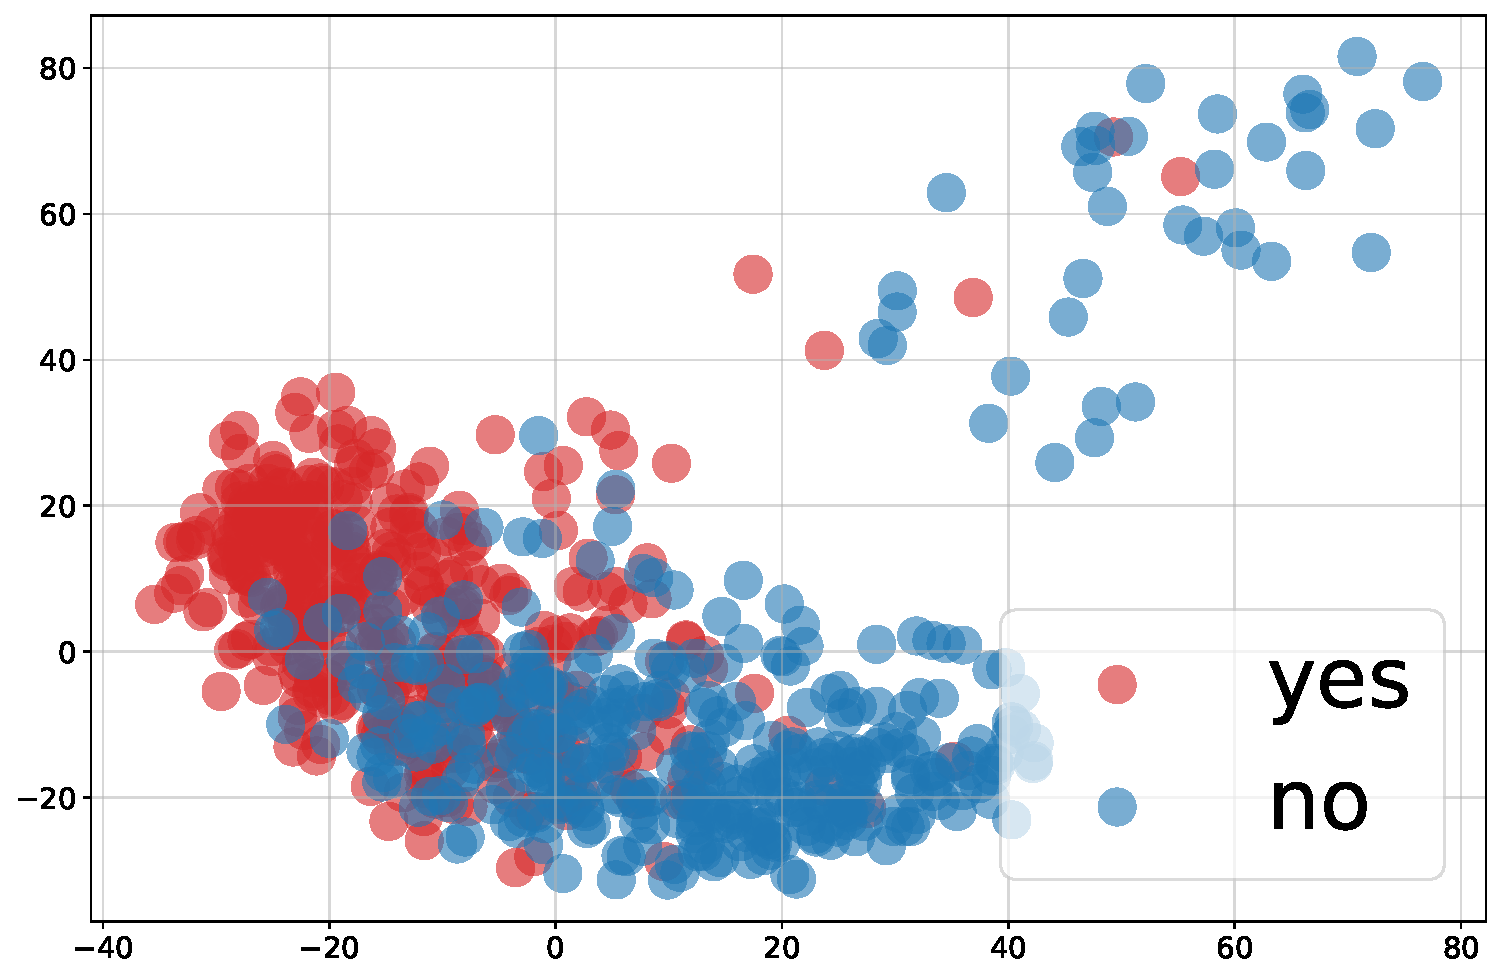
\includegraphics[width=1.0\textwidth]{Figures/model_steering/pca/pca_shift_of_means_llava_29_yes_to_no.pdf}
            \caption*{\small{$l=29$}}
        \end{minipage}%
    
\end{minipage}%
\caption{\textbf{Linear separability of concepts features in MLLMs.} We visualize the features related to the concepts \textcolor{BrickRed}{"yes"} and \textcolor{NavyBlue}{"no"} after PCA projections across MLLMs layers.}
\label{fig:model_steering_qual_pca_concepts_samples}
\end{figure}

\subsection{Multimodal LLMs steering framework.} 
\label{sec:model_steering_framework}

\paragraph{Setup.} For a text-generative multimodal model $f: T \times I \rightarrow T$, we aim to modify the model's output $\hat{y}$ to a desired output $\tilde{\bm{y}}$ by applying a shift or steering vector $\bm{v}$ to the residual stream features $\bm{Z}$, without changing the model parameters. The model is evaluated within a visual question-answering (VQA) framework: where each query consists of a question about an input image, and the model generates an answer. This task encompasses a wide range of applications for MLLMs. To measure the effectiveness of our approach in directing the model towards specific answers or answer types, we report the number of generated answers that align with the target output or answer type. Additionally, we aim for targeted steering, ensuring that only specific answer types are influenced. For example, when altering answers from “yes” to “no” within the "yes/no" category, responses to other question types should remain unaffected. This specificity is assessed by monitoring accuracy across answer types and tracking the number of answers from each answer type.
\paragraph{Implementation details.} Experiments are conducted on the widely-used LLaVA model \cite{liu2024improvedllava}, comprising a CLIP image encoder, a two-layer MLP connector, and a 7B Vicuna-1.5 LLM. In the main paper, we focus on VQAv2 dataset \cite{goyal2017makingvqav2}, a visual question-answering corpus with image-question-answer triplets and annotated answer types ("yes/no", "number", and "other"). We provide also experiments on COCO captioning \cite{lin2014microsoft}, which we detail more in App. B. Steering vectors are derived from a subset of the training set, with model performance evaluated on the validation set. Additional experiments and ablation study can be found in App. B. We find that the steering becomes more effective in deeper layers (see \Cref{fig:model_steering_qual_pca_concepts_samples} and App. B), thus we apply it on the last layer for VQAv2.


\begin{table}[h]
    \centering
    \small
    \resizebox{0.7\linewidth}{!}{
        \begin{tabular}{cccc}
        \toprule	 	
            \multirow{2}{*}{Target Type} 
            & \multicolumn{3}{c}{Answers Type}
            \\
            & yes/no
            & number
            & other
            \\
          \cmidrule(lr{8pt}){1-1}  \cmidrule(lr{8pt}){2-4} 
            N/A
            & 366
            & 122
            & 494
            \\
            \midrule
            yes/no
            & \textbf{557}
            & 96
            & 288
            \\
            number
            & 327
            & \textbf{201}
            & 390
            \\
            other
            & 364
            & 115
            & \textbf{501}
            \\
        \bottomrule
        \end{tabular}
        }
        \caption{\textbf{Steering MLLMs answers type.} Number of target answers type increases significantly after steering the model with the corresponding steering vector.}
    \label{tab:model_steering_answer_type}
\end{table}

\subsection{Coarse-grained model steering} 
\label{sec:model_steering_coarse_steering}
In coarse-grained or global steering, the objective is to adjust the model outputs $\hat{y}$ to generally align with a set of target samples (\emph{e.g.}, changing answers type). Given input-output samples, we first extract the answer representations $\bm{B} = {\bm{b}_1, ..., \bm{b}_N}$ at a specified layer $l$ (we drop the layer index for simplicity) from the target sample set. Similarly, we obtain representations for a set of original samples $\bm{A} = {\bm{a}_1, ..., \bm{a}_M}$, for example, randomly drawn from the training set. We then compute the coarse steering vector $\bm{s}_c$ as follows: 
\begin{equation} 
\label{eq:steering_vector_coarse}
\bm{s}^c = \frac{\sum_i^N \bm{b}_i}{N} - \frac{\sum_i^M \bm{a}_i}{M}, \end{equation}
$s_c$ is applied to all the samples in the validation set. For instance, the activations $z_i$ of a sample $x_i$ (at the same layer $l$), are changed as follows:
\begin{equation} 
\label{eq:steering_vector_coarse}
\tilde{\bm{z}}_i = \bm{z}_i + \alpha \bm{s}_c , \quad \bm{z}_i = f_l(x_i),
\end{equation}
where $\alpha$ controls the steering strength and it is set to 1 (we study $\alpha$ in App. B). $\tilde{\bm{z}}$, replaces $\bm{z}$ and becomes the input to the next layer $l+1$.

\paragraph{Experiments.} We steer the model answers towards a particular type among; yes/no, numbers or other (\emph{e.g.} colors, objects). For each target answer type, we compute a steering vector. \Cref{tab:model_steering_answer_type} shows that the number of answer types increases significantly when applying the corresponding steering vector, this validates the efficacy of globally steering the model.





\begin{figure}[!h]
    \centering
    \begin{minipage}{0.9\linewidth}
    \centering
        
        \begin{minipage}{\linewidth}
            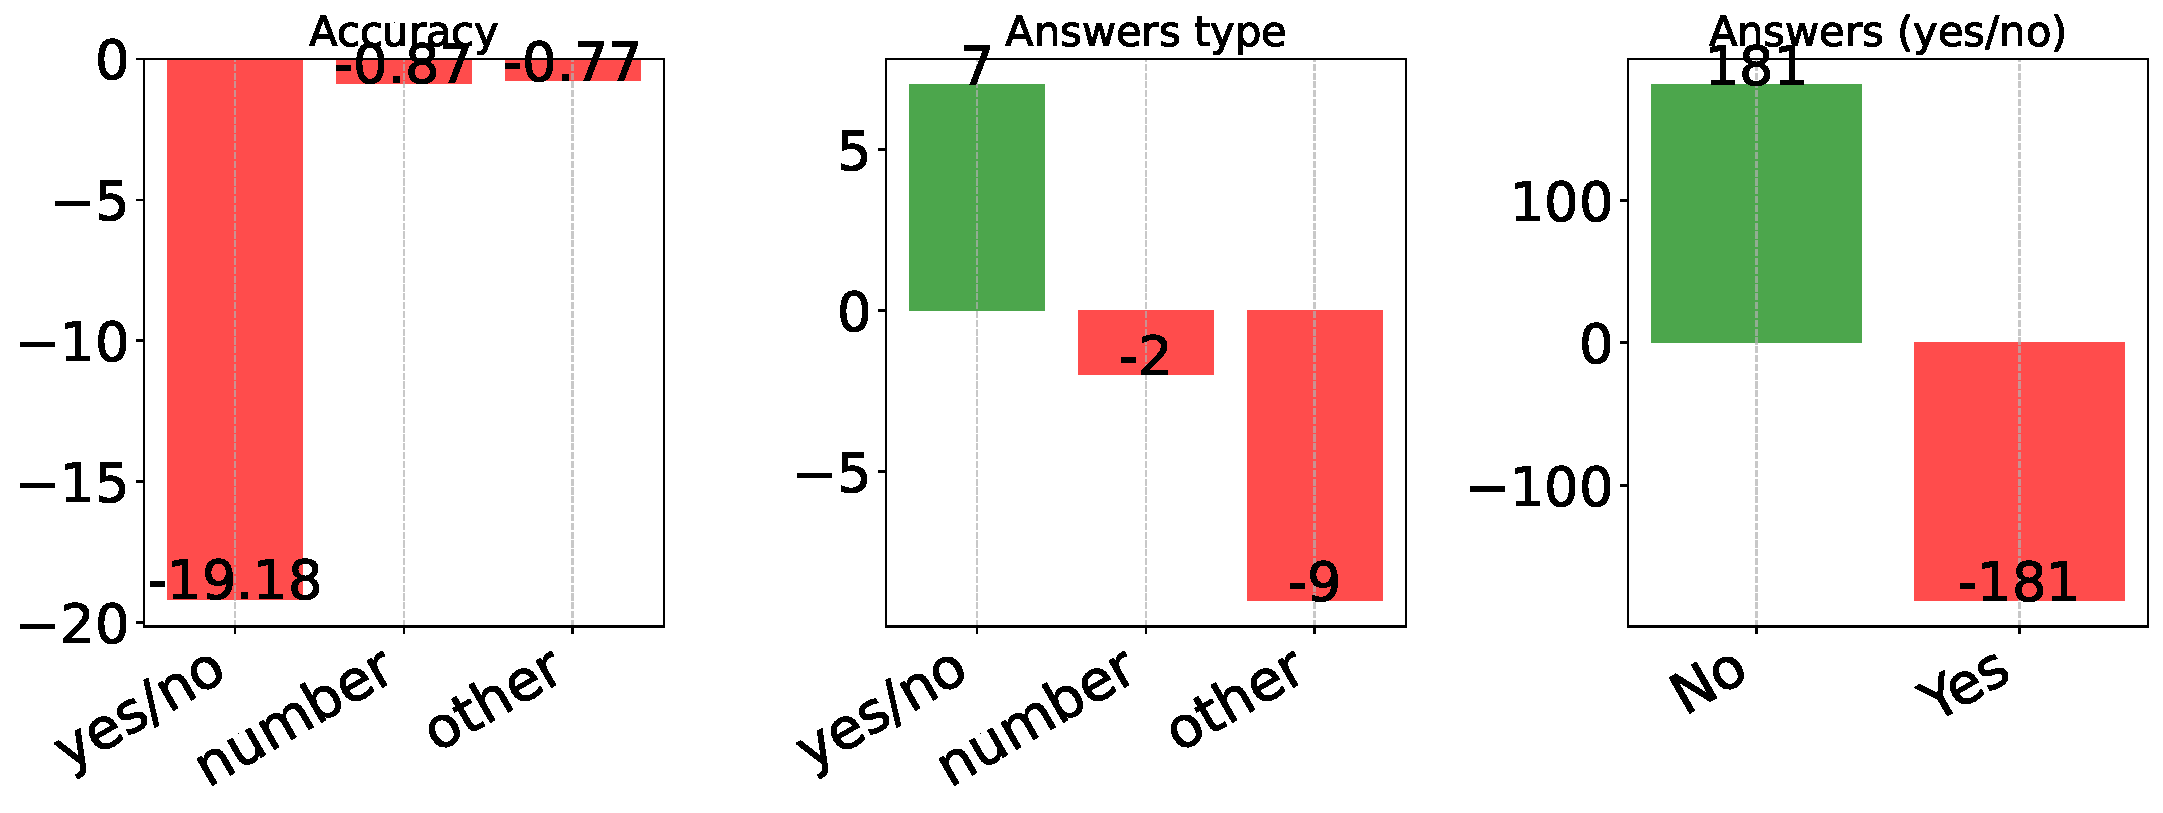
\includegraphics[width=1.0\textwidth]{Figures/model_steering/intra/steering_vector_vqav2_accuracy_llava_type_yes_no_steering_vector_concept_0_to_1_only_target_answers.pdf}
        \end{minipage}%
        
        
        
        \begin{minipage}{\linewidth}
            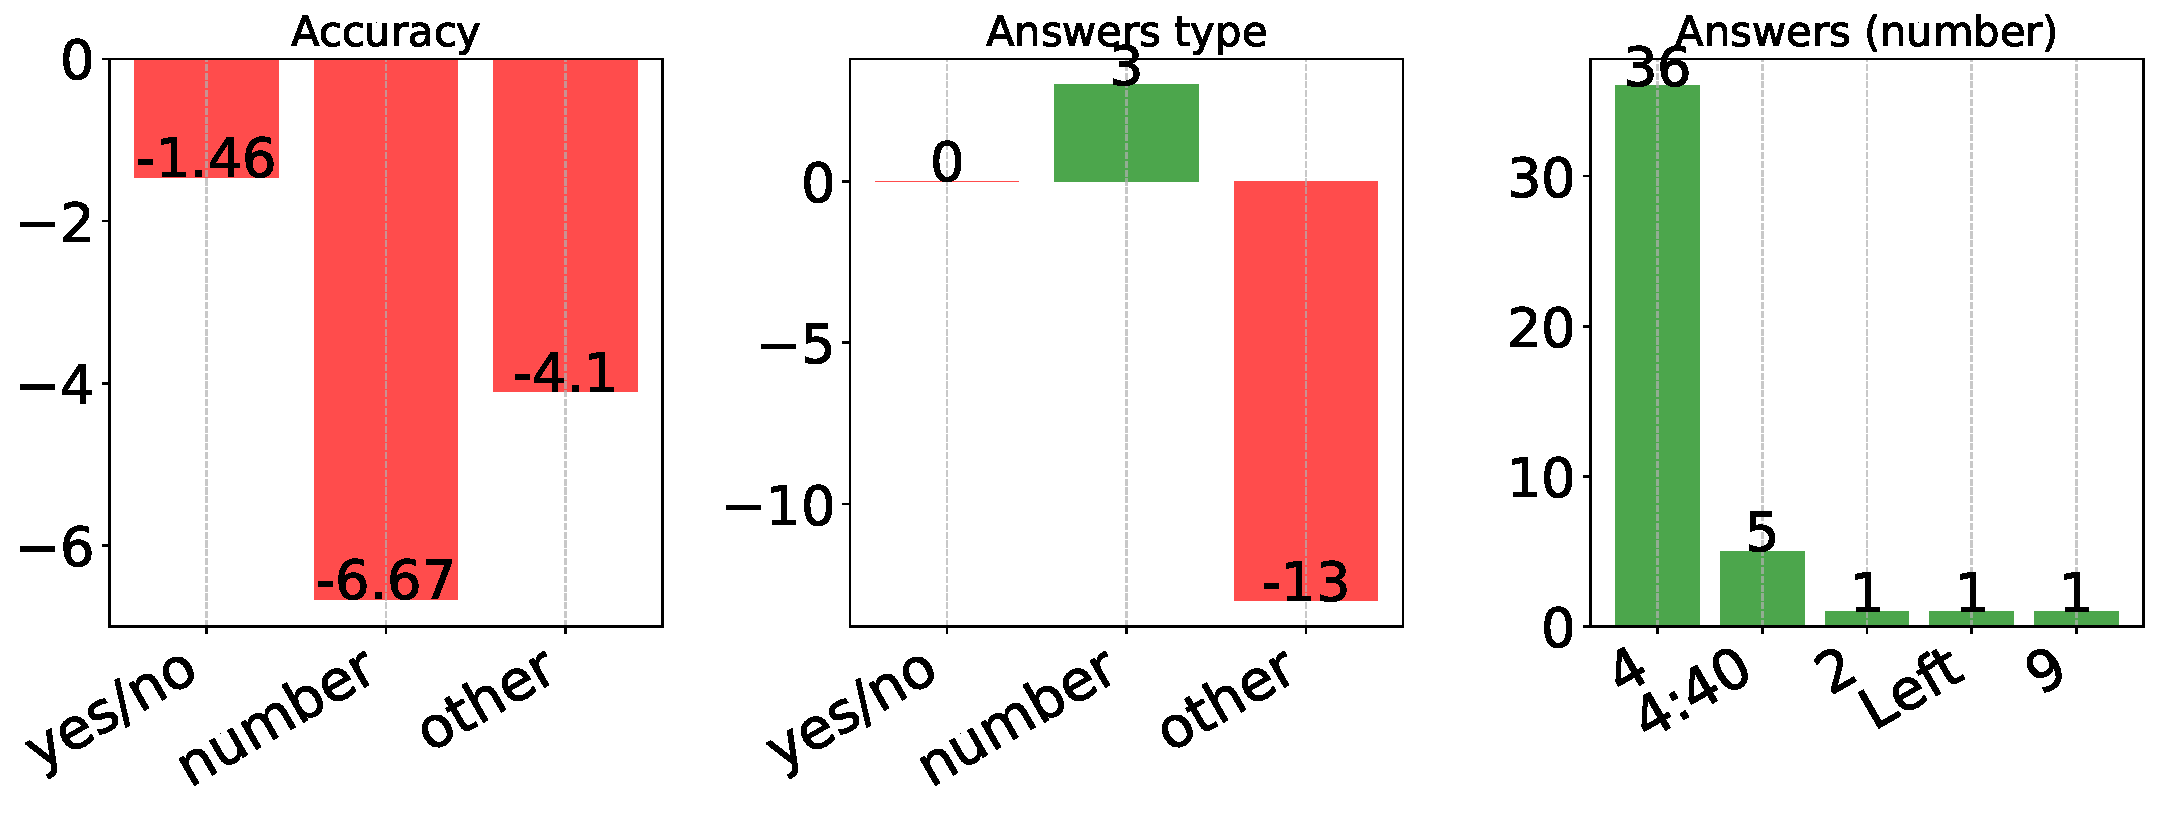
\includegraphics[width=1.0\textwidth]{Figures/model_steering/intra/steering_vector_vqav2_accuracy_llava_type_number_steering_vector_concept_0_to_2_only_target_answers.pdf}
        \end{minipage}%
        
        
        \begin{minipage}{\linewidth}
            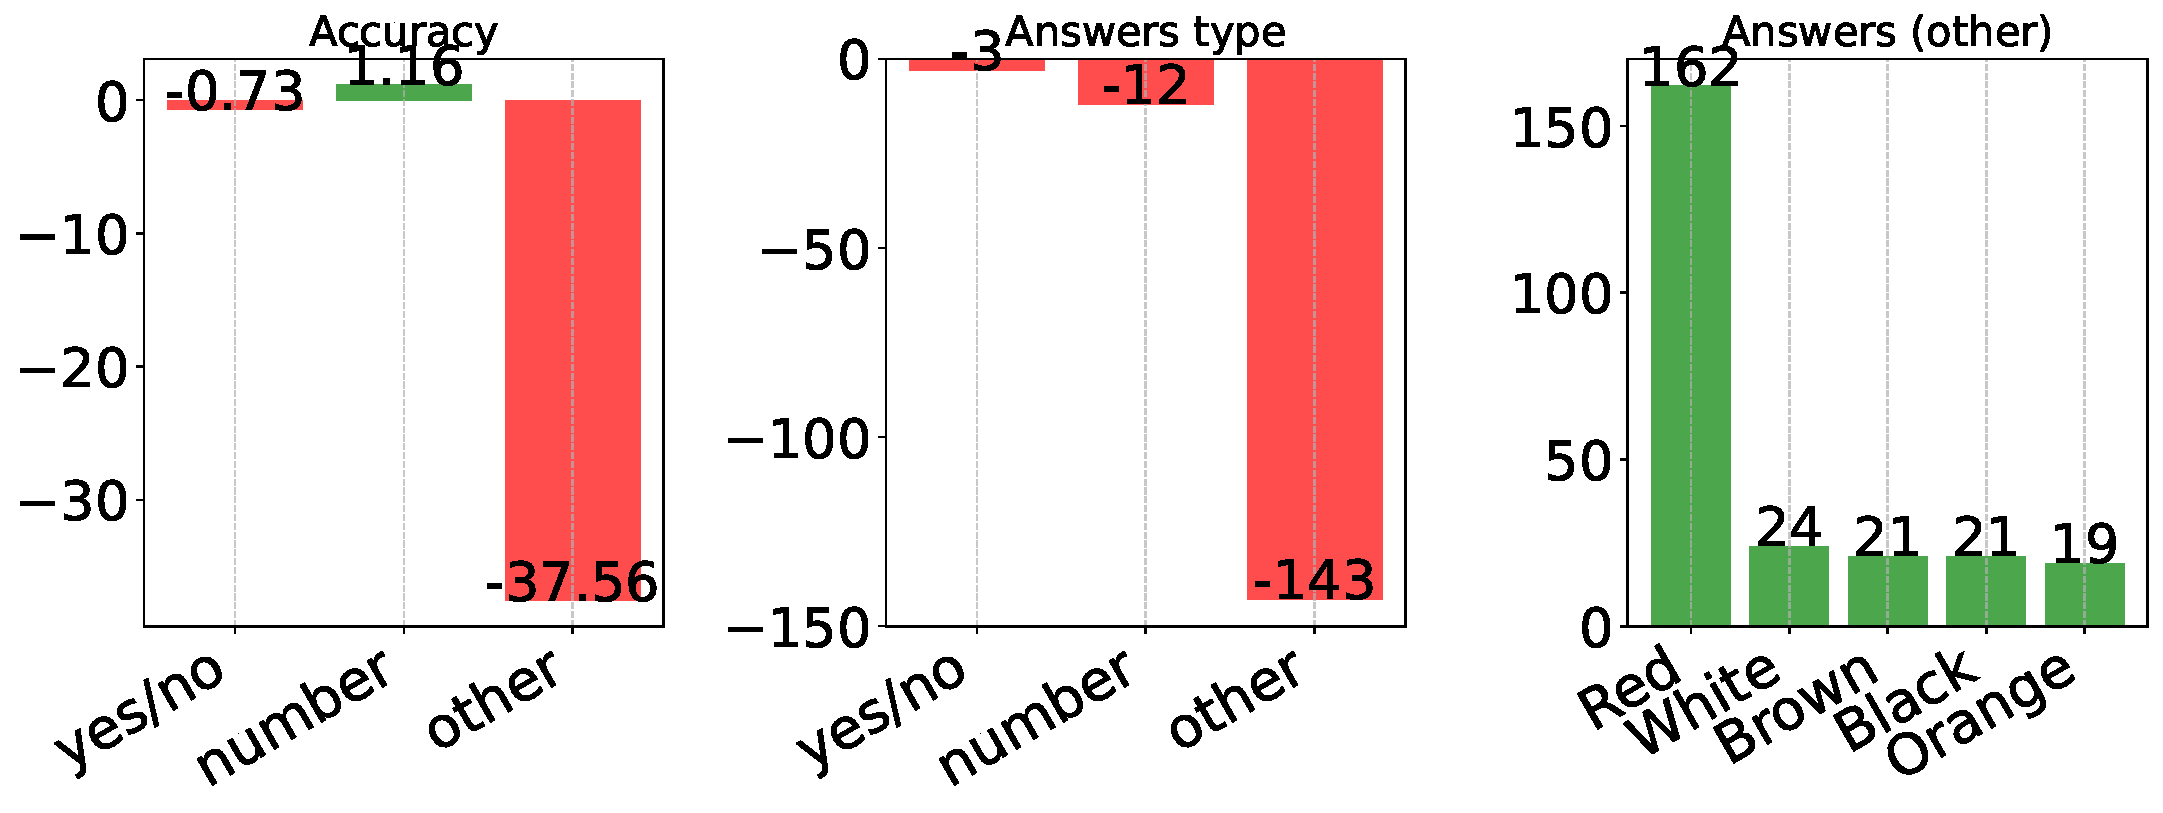
\includegraphics[width=1.0\textwidth]{Figures/model_steering/intra/steering_vector_vqav2_accuracy_llava_type_other_steering_vector_concept_4_to_9_only_target_answers.pdf}
        \end{minipage}%
        
        
    \end{minipage}%
\caption{\textbf{Discovering meaningful steering directions.} Each line corresponds to a fine-grained steering direction to steer the model answer to: "No" (yes/no), "4" (number) and "Red" (other). Some steering directions are targeted (\emph{e.g.}, "No") as there is slight change in both the accuracy on other types (\emph{e.g.}, number, other) and the number of answers type. We show the relative scores compared to a baseline with no steering.}
\label{fig:model_steering_intra}
\end{figure}




\subsection{Discovering meaningful and fine-grained steering directions.}
\label{sec:model_steering_discovering}

Unlike global steering, fine-grained steering focuses on adjusting outputs at the concept level. Specifically, we seek editing directions that adjust only certain concepts. To do this, we decompose the hidden states of a set of samples into a set of concepts $\bm{U}$. We then compute a series of fine-grained steering vectors $\bm{s}^f = {\bm{s}_{11}^f, ..., \bm{s}_{NN}^f}$, where each $\bm{s}_{ij}^f$ represents the steering vector from concept $\bm{u}_i$ to $\bm{u}_j$:

\begin{equation} 
\label{eq:steering_vector_finegrained}
\bm{s}_{ij}^f = \bm{u}_j - \bm{u}_i.
\end{equation}



However, not all computed vectors are necessarily meaningful steering vectors. We identify these vectors based on the strongest impact on guiding the model towards generating specific answers or concepts (\emph{e.g.} producing significantly more target answers). This is more detailed in App. B.

\paragraph{Experiments.} \Cref{fig:model_steering_intra} illustrates some steering vectors. We try to find the steering vectors between concepts decomposed from 3 sample sets corresponding to: "yes/no", "number" and "other" answers type. We notice that some vectors correspond to answering "No", "4" and "Red". This validates the possibility of finding fine-grained steering vectors that can steer the model towards a specific answer.



            




\begin{table}[h]
    \centering
    \small
    \resizebox{1\linewidth}{!}{
        \begin{tabular}{lcccccccc}
        \toprule	 	
            \multirow{2}{*}{Steering} 
            & \multicolumn{3}{c}{Accuracy (\%)} 
            & \multicolumn{3}{c}{Answer Types} 
            & \multicolumn{2}{c}{Answers} \\
            \cmidrule(lr{8pt}){2-4}  
            \cmidrule(lr{8pt}){5-7} 
            \cmidrule(lr{8pt}){8-9}
            & Yes/No 
            & Number 
            & Other 
            & Yes/No 
            & Number 
            & Other 
            & Original 
            & Target \\
        \midrule
            N/A 
            & 90.82 
            & 58.47 
            & 71.10 
            & 1861 
            & 687 
            & 2349 
            & 0 
            & 0 \\
            Yes $\rightarrow$ No 
            & 69.03 
            & 56.82 
            & 68.99 
            & 1884 
            & 695 
            & 2294 
            & -828 
            & +828 \\
            1 $\rightarrow$ 3 
            & 90.71 
            & 54.52 
            & 71.12 
            & 1861 
            & 670 
            & 2350 
            & -215 
            & +144 \\
            White $\rightarrow$ Black 
            & 90.40 
            & 58.42 
            & 58.36 
            & 1861 
            & 671 
            & 2312 
            & -98 
            & +441 \\
        \bottomrule
        \end{tabular}
    }
    \caption{\textbf{Steering MLLMs answers.} Steering answers from "Yes" (Yes/No), "1" (Number), "White" (Other) to "No", "3", "Black" respectively. The number of original/target answer counts decreases/increases significantly, while the accuracy on other answer types changes slightly, and the number of answer type counts remains almost constant.}
    \label{tab:model_steering_answers}
\end{table}



\subsection{Steering towards a specific target answer}\label{sec:model_steering_towards_specific_answers}
Motivated by the previous section, the objective here is to steer the model towards a specific answer specified by the user. For each pair of original/target answers (\emph{e.g.}, yes/no), we collect few hundred samples and compute the steering vector (as in \Cref{sec:model_steering_coarse_steering}). Then we apply the vectors on all samples in the validation set. In \Cref{tab:model_steering_answers}, we report the evaluation metrics when targeting the last layer. We can notice that the steering is effective as the number of target answers increase, while the accuracy on other answer types only slightly changes.

\begin{figure}[!h]
    \centering
    \begin{minipage}{\linewidth}
    \centering
        \begin{minipage}{\linewidth}
            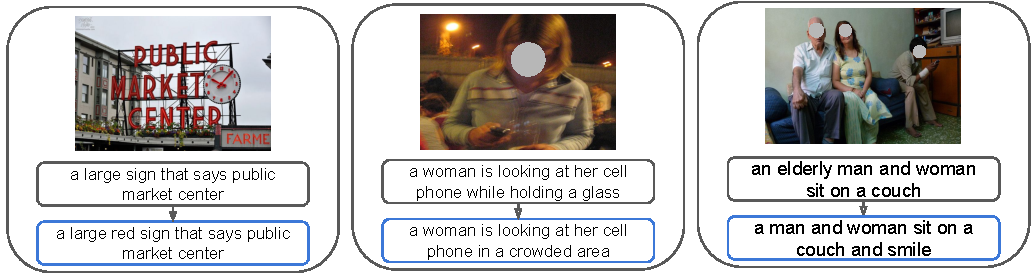
\includegraphics[width=1.0\textwidth]{Figures/model_steering/qualitative/model_steering_change_captions_type_main.pdf}
        \end{minipage}%
    \end{minipage}%
\caption{\textbf{Steering MLLMs captions style.} Captions \textcolor{blue}{steered} to focus more on colors (left), places (middle) and sentiments (right).}
\label{fig:model_steering_captions_style_main}
\end{figure}

\subsection{Steering image captions}
\label{sec:model_steering_captions_type}

In our earlier experiments, we applied steering on relatively brief answers from the VQAv2 dataset. Here, we extend this approach to longer, descriptive outputs using the COCO image captioning dataset \cite{lin2014microsoft}. Given that multiple captions can effectively describe an image by emphasizing various aspects such as the main object, surroundings, actions, or events, our focus is modifying captions to align with a specific target style (see \Cref{fig:model_steering_captions_style_main}). We presents the results in \Cref{tab:model_steering_captions_type}, demonstrating that captions can be steered towards a target style so that they focus more on places, colors, or sentiments. These findings validate the feasibility of steering MLLMs on tasks with longer responses.


\begin{table}[h]
    \centering
    \small
    \resizebox{0.7\linewidth}{!}{
        \begin{tabular}{cccc}
        \toprule	 	
            \multirow{2}{*}{Target Style} 
            & \multicolumn{3}{c}{Captions Style}
            \\
            & places
            & colors
            & sentiments
            \\
          \cmidrule(lr{8pt}){1-2}  \cmidrule(lr{8pt}){2-4} 
            N/A
            & 430
            & 1309
            & 2
            \\
            \midrule
            places
            & \textbf{796}
            & 1077
            & 1
            \\
            colors
            & 488
            & \textbf{2561}
            & 1
            \\
            sentiments
            & 393
            & 1040
            & \textbf{48}
            \\
        \bottomrule
        \end{tabular}
        }
        \caption{\textbf{Steering MLLMs captions style.} Each line corresponds to different steering vector. Steering towards a target style increases the number of captions with that style.}
    \label{tab:model_steering_captions_type}
\end{table}
